\chapter{\LTLf and \LDLf}
\label{ch:logic}
%In this chapter we describe the background knowledge required for this work. We introduce Markov Decision Process (MDP) and Non-Markovian Reward Decision Process (NMRDP), common formalisms in the context of Reinforcement Learning. We describe Linear Temporal Logic over finite traces (\LTLf) and Linear Dynamic Logic over finite traces (\LDLf), that we use for define temporal goal in an RL setting. Then, we describe an important result about RL for NMRDP with \LTLf/\LDLf rewards, that is the basis for this work.

In this chapter, we introduce the reader to the main important framework to talk about behaviours over time, which gives the foundations for our approach.
First, we talk about the well-known Linear-Time Temporal Logic (\LTL), Propositional Dynamic Logic (\PDL) and their main applications; then we go more in deep by presenting a specific formalism, namely \emph{Linear Temporal Logic over Finite Traces} \LTLf and \emph{Linear Dynamic Logic over Finite Traces} \LDLf. Finally, we study the translation from \LLf formulas to Deterministic Finite Automata (\DFA).
We require the reader to be acquainted with classical logic \citep{sep-logic-classical} and automata theory \citep{Hopcroft:2000:IAT:557657}.
\section{Linear-time Temporal Logic (\LTL)}\label{sect:ltl}
\emph{Temporal Logic} \citep{sep-logic-temporal} is a category of formal languages aimed to talk about properties of a system whose truth value might change over time. This is in contrast with atemporal logics, which can only discuss statements whose truth value is constant. 

\emph{Linear time Temporal Logic} \citep{Pnueli:1977:TLP:1382431.1382534}, or \emph{Linear Temporal Logic} (\LTL) is such a logic. It is the most popular and widely used temporal logic in computer science, especially in formal verification of software/hardware systems, in AI to reasoning about actions and planning, and in the area of Business Process Specification and Verification to specify processes declaratively.

It allows to express temporal patterns about some property $p$, like \emph{liveness} (\emph{$p$ will eventually happen}), \emph{safety} (\emph{$p$ will never happen}) and \emph{fairness}, combinations of the previous patterns (\emph{infinitely often $p$ holds}, \emph{eventually always $p$ holds}).

\subsection{Syntax}\label{sect:ltl-syntax}
A \LTL formula $\varphi$ is defined over a set of propositional symbols $\Prop$ and are closed under the boolean connectives, the unary temporal operator \Next (\emph{next-time}) and the binary operator $\lUntil$ (\emph{until}):

\[\begin{array}{rcl}
\varphi &::=& A \mid \lnot \varphi \mid \varphi_1\land \varphi_2 \mid \Next\varphi \mid \varphi_1 \lUntil \varphi_2
\end{array}
\]
With $A\in \Prop$.

Additional operators can be defined in terms of the ones above: as usual logical operators such as $\lOR, \Rightarrow, \Leftrightarrow, \true, \false$ and temporal formulas like \emph{eventually} as $\Diamond \varphi \doteq \true \lUntil \varphi$, \emph{always} as $\Box \varphi \doteq \lnot \Diamond \lnot \varphi$ and \emph{release} as $\varphi_1 \Release \varphi_2 \doteq \lnot (\lnot \varphi_1 \lUntil \lnot \varphi_2)$.

\begin{example}\label{ltl-formula-examples}
Several interesting temporal properties can be defined in \LTL:
\begin{itemize}
	\item \emph{Liveness}: $\Diamond \varphi$, which means "condition expressed by $\varphi$ \emph{at some time} in the future will be satisfied", "sooner or later $\varphi$ will hold" or "eventually $\varphi$ will hold". E.g., $\Diamond rich$ (eventually I will become rich), $Request \implies \Diamond Response$ (if someone requested the service, sooner or later he will receive a response).
	\item \emph{Safety}: $\Box \varphi$, which means "condition expressed by $\varphi$, \emph{every time} in the future will be satisfied", "always $\varphi$ will hold". E.g., $\Box happy$ (I'm always happy), $\Box \lnot (temperature >30)$ (the temperature of the room must never be over 30).
	\item \emph{Response}: $\Box \Diamond \varphi$ which means "at any instant of time there exists a moment later where $\varphi$ holds". This temporal pattern is known in computer science as \emph{fairness}.
	\item \emph{Persistence}: $\Diamond \Box \varphi$, which stand for "There exists a moment in the future such that from then on $\varphi$ always holds". E.g. $\Diamond \Box dead$ (at a certain point you will die, and you will be dead forever)
	\item \emph{Strong fairness}: $\Box \Diamond \varphi_1 \implies \Box \Diamond \varphi_2$, "if something is attempted/requested infinitely often, then it will be successful/allocated infinitely often". E.g., $\Box \Diamond ready \implies \Box \Diamond run$ (if a process is in ready state infinitely often, then infinitely often it will be selected by the scheduler).
\end{itemize}
\end{example}

\subsection{Semantics}\label{ltl-semantics}
The semantics of \LTL is provided by (infinite) \textit{traces}, i.e. $\omega$-word over the alphabet $2^\Prop$.  


\begin{definition}\label{ltl-satisfaction}
	Given a infinite trace $\trace$, we define that a \LTL formula $\varphi$ is \emph{true} at time $i$, in symbols $\trace, i \models \varphi$ inductively as follows:
	\begin{align*}
	\trace, i &\models A, \tm{for} A\in\Prop \tiff A \in \trace(i)\\
	\trace, i &\models \lnot \varphi \tiff \trace, i \not\models \varphi\\
	\trace, i &\models \varphi_1 \lAND \varphi_2 \tiff \trace, i \models \varphi_1 \lAND \trace, i \models \varphi_2\\
	\trace, i &\models \Next\varphi \tiff \trace,i+1 \models \varphi\\
	\trace, i &\models \varphi_1 \lUntil \varphi_2 \tiff \exists j. (j\ge i) \lAND \trace,j \models \varphi \lAND\forall k. (i\le k < j) \Rightarrow \trace, k \models \varphi_1\\
	\end{align*}
\end{definition}
Similarly as in classical logic we give the following definitions:
\begin{definition}\label{ltl-sat-val-ent}
	A \LTL formula is \emph{true} in $\trace$, in notation $\trace \models \varphi$, if $\trace, 0 \models \varphi$. A formula $\varphi$ is \emph{satisfiable} if it is true in some $\trace$ and is \emph{valid} if it is true in every $\trace$. $\varphi_1$ \emph{entails} $\varphi_2$, in symbols $\varphi_1 \models \varphi_2$ iff $\forall \trace, \forall i.\trace, i \models \varphi_1 \implies \trace, i \models \varphi_2$.
\end{definition}

Now we state an important result:
\begin{theorem}[\cite{Sistla:1985:CPL:3828.3837}]
	Satisfiability, validity, and entailment for \LTL formulas are \PSPACE-complete.
\end{theorem}
Indeed, Linear Temporal Logic can be thought of as a specific decidable (\PSPACE-complete) fragment of classical first-order logic (\FOL).

Notice that, a \emph{trace} $\trace$ can be seen as a \emph{word} on a \emph{path} of a \emph{Kripke structure}.
\begin{definition}[\cite{Clarke:2000:MC:332656}]\label{kripke}
	a Kripke structure $\Kripke$ over a set of propositional symbols $\Prop$ is a 4-tuple $\tup{\States, I, R, L}$ where $\States$ is a finite set of \emph{states}, $I\subseteq \States$ is the set of \emph{initial states}, $R \subseteq \States \times \States$ is the \emph{transition relation} such that $R$ is left-total and $L: \States \to 2^\Prop$ is a \emph{labeling function}.
\end{definition}
A \emph{path} $\rho$ over $\Kripke$ is a sequence of states $\tup{s_1, s_2, \dots}$ such that $\forall i. R(s_i, s_{i+1})$. From a path we can build a \emph{word} $w$ on the path $\rho$ by  
mapping each state of the sequence with $L$, namely:
\[
w = \tup{L(s_1), L(s_2), \dots}
\]

In simpler words, a trace of propositional symbols $\Prop$ is a infinite sequence of combinations of propositional symbols in $\Prop$. Moreover, we denote by $\trace(i)$ with $i\in\Naturals$ the labels associated to $s_i$, i.e. $L(s_i)$.
\begin{example}\label{kripke-example}
	In figure \ref{kripke-fig-example} is depicted an example of Kripke structure $\Kripke$ over $\Prop = \{p, q\}$ where:
	\begin{align*}
	\States &= \{s_1, s_2, s_3\}\\
	I &= \{s_1\}\\
	R &= \{(s_1, s_2), (s_2, s_1), (s_2, s_3), (s_3, s_3)\}\\
	L &= \{(s_1, \{p, q\}), (s_2, \{q\}), (s_3, \{p\})\}
	\end{align*}
	 
	\begin{figure}[h]
		\centering	
		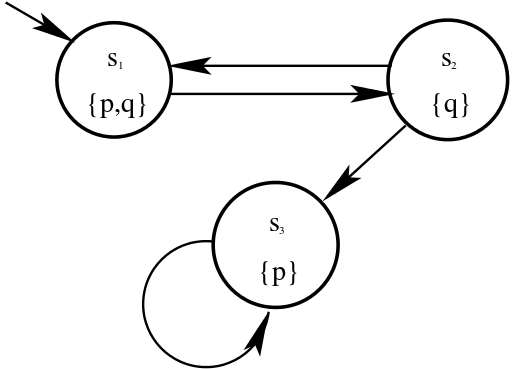
\includegraphics[width=.5\linewidth]{images/KripkeStructureExample}
		\caption{\label{kripke-fig-example}An example of Kripke structure.}
	\end{figure}
	
	The path $\tup{s_1, s_2, s_3, s_3, s_3\dots}$ yields the following trace $\trace$:
	\begin{align*}
	\trace &= \tup{L(s_1), L(s_2), L(s_3), L(s_3), L(s_3),\dots} \\
		&= \tup{\set{p, q}\set{q}, \set{p}, \set{p},\set{p}, \dots}
	\end{align*}
\end{example}




%\section{Propositional Dynamic Logic (\PDL)}\label{pdl}
%\emph{Dynamic Logics} \citep{Pratt:1976:SCF:889769, sep-logic-dynamic} (\DL) are modal logics\footnote{\emph{Modal Logic} extends classical logics to include operator  expressing \emph{modality} (e.g. "necessarily", "possibly", "usually"). However, the term "modal logic" is used more broadly to cover a family of logics with similar rules and a variety of different symbols. Temporal Logic and Dynamic Logic described in this chapter are examples of modal logics. \citep{sep-logic-modal}}
%for representing the states and the events of dynamic systems. We can speak about the properties that holds in a state (assertion language) and about properties on transitions between states (programming language). Dynamic Logics are indeed called \emph{logics of programs.}
%
%Propositional Dynamic Logic \citep{FISCHER1979194} (\PDL), probably the most well-known (propositional) logic of programs in computer science, is the propositional counterpart of Pratt's original dynamic logic \citep{Pratt:1976:SCF:889769}, which was a \emph{first-order} modal logic. Basically, this means that from three types of terms, \emph{assertions}, \emph{data} (as in \FOL) and \emph{actions} we drop the \emph{data} terms, hence we can reason only about abstract propositions and the actions for modify them.
% 
%As we did with \LTL, in the following sections we describe syntax and semantics of \PDL.
%\subsection{Syntax}\label{pdl-syntax}
%A \PDL formula $\varphi$ is defined over a set of propositional symbols $\Prop$ and a set of atomic programs $\Pi$ built as follows:
%
%\[\begin{array}{lcl}
%\varphi &::=& A \mid \bZero  \mid \lnot \varphi \mid \varphi_1 \land \varphi_2 \mid \BOX{\alpha}\varphi \\
%\alpha &::=& \phi \mid \varphi? \mid  \alpha_1 + \alpha_2 \mid \alpha_1; \alpha_2 \mid \varrho^*
%\end{array}
%\]
%with $A\in \Prop$ and $\phi \in \Pi$.
%We can define classical logic operators $\lOR, \Rightarrow, \Leftrightarrow, \bOne$ as usual, and the \emph{possibility} operator $\DIAM{\ }$ from the \emph{necessity} operator $\BOX{\ }$, namely $\DIAM{\alpha}\varphi \doteq \lnot \BOX{\alpha}\lnot \varphi$. The propositions $\BOX{\alpha}\varphi$ and $\DIAM{\alpha}\varphi$ are read "box $\alpha$ $\varphi$" and "diamond $\alpha$ $\varphi$", respectively. 
%
%Notice that $\varphi$ stands for the propositional component of the logic, while program $\alpha$ stands for the dynamic component. Moreover, notice that propositions and programs are intertwined and cannot be separated: the definition of propositions depends on the definition of programs because of the construct $\BOX{\alpha}\varphi$, and the definition of programs depends on the definition of propositions because of the construct $\varphi?$. 
%
%\begin{example}
%	Now we provide some example of compound formulas and programs:
%	\begin{itemize}
%		\item $\BOX{\alpha}\varphi$: "It is necessary that after executing $\alpha$, $\varphi$ is true";
%		\item $\DIAM{\alpha}\varphi$ "There exists a computation of $\alpha$ that terminates in a state satisfying $\varphi$.
%		\item $\alpha;\beta$: "Execute $\alpha$, then execute $\beta$";
%		\item $\alpha; \cup \beta$: "Choose either $\alpha$ or $\beta$ nondeterministically and execute it";
%		\item $\alpha^*$: "Choose $\alpha$ a nondeterministically chosen finite number of times (zero or more);
%		\item $\varphi?$: "Test $\varphi$: proceed if true, fail if false".
%	\end{itemize}
%\end{example}
%
%\begin{example}
%	To better understand the expressive power of \PDL, it is worth to notice this correspondence between basic programming language constructs and \PDL formulas:
%	\begin{align*}
%		\mathbf{skip} &\defeq \bOne \\
%		\mathbf{fail} &\defeq \bZero \\
%		\mathbf{if\ \varphi\ then\ \alpha\ else\ \beta} &\defeq \varphi?;\alpha \cup \lnot \varphi?;\beta \\
%		\mathbf{while\ \varphi\ do\ \alpha} &\defeq (\varphi?;\alpha)^*;\lnot\varphi?\\
%		\mathbf{repeat\ \alpha\ until\ \varphi} &\defeq \alpha;(\lnot\varphi?;\alpha)^*;\varphi?\\
%		\set{\varphi} \alpha \set{\psi} &\defeq \varphi \implies \BOX{\alpha}\varphi\\
%	\end{align*}
%	The programs \textbf{skip} and \textbf{fail} are the program that does nothing (no-op) and the failing program, respectively. The ternary \textbf{if-then-else} operator and the binary \textbf{while-do} operator are the usual conditional and while loop constructs found in conventional programming languages. The	construct $\set{\varphi} \alpha \set{\psi}$ is the Hoare partial correctness assertion \citep{4567894}.
%\end{example}
%\subsection{Semantics}
%The semantics for \PDL formulas is provided by \emph{Labelled Transition System} (\LTS). 
%%Here we give a definition that encompasses Definition \ref{kripke}, by giving meaning also on transitions.
%\begin{definition}
%	A \emph{Labelled Transition System} over a set of propositional symbols $\Prop$ and a set of atomic programs $\Pi$ is a 3-tuple $\tup{\States, R_p, V}$ where $\States$ is the set of \emph{states}, $R_p: \Pi \to 2^{\States \times \States}$ is a mapping from atomic programs to a binary relation over $\States$ and $V: \Prop \to 2^{\States}$ is a mapping from propositional symbols to subsets of $\States$.
%\end{definition}

%\begin{example}\label{lts-example}
%	In figure \ref{lts-figure} two examples of \LTS defined over $\Prop = \set{p, q}$ and $\Pi = \set{\pi_1,\pi_2}$ are depicted. For the \LTS on the left, $\M_1$,  we have:
%	\begin{align*}
%	\States &= \set{x_1, x_2}\\
%	R_p(\pi_1) &= \set{(x_1, x_1)}\\
%	R_p(\pi_2) &= \set{(x_1, x_2)}\\
%	V(p) &= \set{x_1}\\
%	V(q) &= \set{x_2}\\	
%	\end{align*}
%	While for the \LTS on the right, $\M_2$,  we have:
%	\begin{align*}
%	\States &= \set{y_1, y_2, y_3, y_4}\\
%	R_p(\pi_1) &= \set{(y_1, y_2), (y_2, y_2)}\\
%	R_p(\pi_2) &= \set{(y_1, y_3), (y_2, y_4)}\\
%	V(p) &= \set{y_1, y_2}\\
%	V(q) &= \set{y_3, y_4}\\
%	\end{align*}
%	\begin{figure}[h]
%		\centering	
%		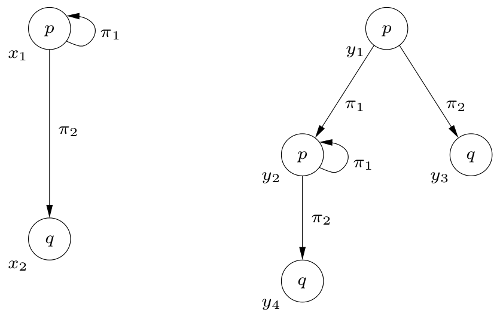
\includegraphics[width=.8\linewidth]{images/bisimilar-LTS-tras}
%		\caption{\label{lts-figure}Two examples of \LTS}
%	\end{figure}
%\end{example}

%In order to formally define the semantics of a \PDL formula $\varphi$, we use the following notation: 
%\begin{itemize}
%	\item $x R(\pi) y$ iff there exists an execution of $\pi$ from $x$ that leads to $y$;
%	\item $x \in V(p)$ iff $p$ is true in $x$.
%\end{itemize}
%In order to include all possible propositions and programs, we extend $R_p$ and $V$ inductively as follows:
%\begin{itemize}
%	\item $xR_p(\alpha;\beta)y$ iff there exists a state $z$ such that 	$xR_p(\alpha)z$ and $zR_p(\beta)y$
%	\item $	xR_p(\alpha \cup \beta)y$ iff $xR_p(\alpha)y$ and $xR_p(\beta)y$
%	\item $	xR_p(\alpha*)y$ iff there exists an integer $n$ and there exist states $z_0,\dots, z_n$ such that $z_0=x, z_n=y$ and $\forall.k= 1, \dots, n$,  $z_{k-1}R_p(\alpha)z_k$
%	\item $	xR_p(\varphi?)y$ iff $x = y \lAND y \in V(\varphi)$
%	\item $V(0) = \emptyset $
%	\item $V(\lnot \varphi)$ = $\States \setminus V(\varphi)$
%	\item $	V(\varphi_1 \lAND \varphi_2) = V(\varphi_1) \lAND V(\varphi_2)$,
%	\item $	V([\alpha]\varphi) = \set{x| \forall y.y \in \States \lAND xR_p(\alpha)y \implies y \in V(\varphi)}$
%\end{itemize}
%Now we give a definition for \PDL formula satisfaction as we did in Definition \ref{ltl-satisfaction}:
%
%\begin{definition}
%	Given a \LTS $\M$, we define that a \PDL formula $\varphi$ is \emph{true in a state $s$}, in symbols $\M, s \models \varphi$ iff $s\in V(\varphi)$:
%\end{definition}

%\begin{example}
%	Considering $\M_1$ and $\M_2$ introduced in Example \ref{lts-example}, we can give the following statements:
%	\begin{itemize}
%		\item $\M_1, x_1 \models p$
%		\item $\M_1, x_2 \models q$
%		\item $\M_1, x_1 \models \DIAM{\pi_1}p \lAND \DIAM{\pi_2}q$
%		\item $\M_1, x_1 \models \BOX{\pi_1^*}p$
%		\item $\M_2, y_1 \models \DIAM{\pi_1^*; \pi_2}q$
%		\item $\M_2, y_1 \models \BOX{\pi_1 \cup \pi_2}(q\lOR p)$
%		\item $\M_2, y_3 \models \BOX{\pi_1 \cup \pi_2}\mathbf{0}$
%	\end{itemize}
%\end{example}

%\begin{definition}
%We define \emph{satisfiability}, \emph{validity} and \emph{entailment} for \PDL formulas in an analogous fashion as we did for \LTL formulas in Definition \ref{ltl-sat-val-ent}.
%\end{definition}
%Now we cite a result about complexity of reasoning in \PDL:
%
%\begin{theorem}[\cite{PRATT1980231}]
%	\emph{satisfiability}, \emph{validity} and \emph{entailment} in \PDL is \EXPTIME-complete.
%\end{theorem}
%In \citep{deGiacomo:2000:CDM:359243.359271} has been proposed an algorithm more effective in practice, though still running in deterministic exponential time in the worst case.

\section{Linear Temporal Logic on Finite Traces: \LTLf}
\label{ltlf}
Linear-time Temporal Logic over finite traces, \LTLf, is essentially standard 
\LTL \citep{Pnueli:1977:TLP:1382431.1382534} interpreted over finite, instead of over infinite, traces \citep{de2013linear}.
This apparently trivial difference has a big impact: as we will see, some \LTL formula has a different meaning if interpreted over infinite traces or finite ones.

\subsection{Syntax}\label{ltlf-syntax}
In fact, the syntax of \LTLf is the same of the one showed in Section \ref{sect:ltl-syntax}, i.e. \emph{formulas} of \LTLf are built from a set $\Prop$ of propositional symbols and are closed under the boolean connectives, the unary temporal operator \Next (\emph{next-time}) and the binary operator $\lUntil$ (\emph{until}):

\[\begin{array}{rcl}
\varphi &::=& \phi \mid \lnot \varphi \mid \varphi_1\land \varphi_2 \mid \Next\varphi \mid \varphi_1 \lUntil \varphi_2
\end{array}
\]
With $A\in \Prop$.

We use the standard abbreviations for classical logic formulas:
\begin{align*}
	\varphi_1\lor\varphi_2 &\doteq \lnot(\lnot \varphi_1\land \lnot
	\varphi_2)\\
	\varphi_1 \Rightarrow \varphi_2 &\doteq \lnot \varphi_1 \lOR \varphi_2\\
	\varphi_1 \Leftrightarrow \varphi_2 &\doteq \varphi_1 \Rightarrow \varphi_2 \lAND \varphi_2 \Rightarrow \varphi_1\\
	\true  &\doteq \lnot \varphi \lOR \varphi\\
	\false &\doteq \lnot \varphi \lAND \varphi\\
\end{align*}
And for temporal formulas:
\begin{align}
\varphi_1 \Release \varphi_2 &\doteq \lnot (\lnot \varphi_1 \lUntil \lnot \varphi_2) \label{ltlf-release}\\
\Diamond\varphi &\doteq \true\lUntil\varphi \label{ltlf-eve}\\
\Box\varphi &\doteq\lnot\Diamond\lnot\varphi \label{ltlf-alw}\\
\Wnext \varphi &\doteq \lnot \Next \lnot \varphi \label{ltlf-wn}\\
\Last &\doteq \Wnext\false \label{ltlf-last}\\
\Ended &\doteq \Box\false \label{ltlf-ended}
\end{align}
As the reader might already noticed, \ref{ltlf-eve} and \ref{ltlf-alw} are defined as in Section \ref{sect:ltl-syntax};  Equation \ref{ltlf-release} is called \emph{release}; Equation \ref{ltlf-wn} is called \emph{weak next} (notice that on finite traces $\lnot \Next \varphi \not\equiv \Next \lnot \varphi$); \ref{ltlf-last} denotes the end of the trace, while \ref{ltlf-ended} denotes that the trace is ended.
\begin{example}\label{ltlf-formula-examples}
	Here we recall Example \ref{ltl-formula-examples} and we see the impact on \emph{Always}, \emph{Eventually} \emph{Response} and \emph{Persistence} \LTL formulas if interpreted on finite traces (i.e. formulas in \LTLf):
	\begin{itemize}
		\item \emph{Safety}: $\Box A$ means that always \emph{till the end of the trace} $\varphi$ holds;
		\item \emph{Liveness}: $\Diamond A$ means that eventually \emph{before the end of the trace} $\varphi$ holds;
		\item \emph{Response}: $\Box \Diamond \varphi$ on finite
		 traces becomes equivalent to \emph{last point in the trace satisfies $\varphi$}, i.e. $\Diamond(\Last \lAND \varphi)$. Intuitively, this is true because $\Box \Diamond \varphi$ implies that at the last point in the trace $\varphi$ holds (because there are no successive instants of time that make $\varphi$ true); but if this is the case, then what happens at previous points in the trace does not matter because the formula evaluates always to true, since as we just said $\varphi$ must hold at the last point in the trace, hence the equivalence with $\Diamond(\Last \lAND \varphi)$.
		\item \emph{Persistence}: $\Diamond \Box \varphi$ on finite traces becomes equivalent to \emph{last point in the trace satisfies $\varphi$}, i.e. $\Diamond(\Last \lAND \varphi)$. Analogously to the previous case, the equivalence holds because $\Diamond \Box \varphi$ implies that at the last point in the trace $\Box \varphi$ holds (and so $\varphi$) since we have no further successive instants of time that make $\Box \varphi$ true. But if this is the case, then what happens at previous points in the trace does not matter because the formula evaluates always to true, since as we just said $\Box \varphi$ (and so $\varphi$) must hold at the last point in the trace, hence the equivalence with $\Diamond(\Last \lAND \varphi)$.
	\end{itemize}
	In other words, no direct nesting of eventually and always connectives is meaningful in \LTLf, and this contrast what happens in \LTL of infinite traces.
\end{example}

\begin{example}
	Another remarkable evidence about the relevance of the assumption about the finiteness of traces is provided by the \DECLARE approach \citep{Pesic:2006:DAF:2135571.2135592}. 
	
	\DECLARE is a declarative approach to business process modeling based on \LTL interpreted over finite traces. The intuition is to map finite traces describing a domain of interest (e.g. processes) into infinite traces under the assumption that 
	\begin{equation}\label{declare-assumption}
	\Diamond \End \lAND \Box(\End \Rightarrow \Next \End) \lAND \Box (\End \Rightarrow \bigwedge_{p \in \Prop} \lnot p)
	\end{equation}
	which means that the following english statements hold:
	\begin{itemize}
		\item $\End$ eventually holds ($\End \notin \Prop$);
		\item once $\End$ is true, it is true forever;
		\item when $\End$ is true all other propositions must be false
	\end{itemize}
	In other words, every finite trace $\pi_f$ is extended with an infinite sequence of $\End$, or in symbols $\pi_{inf} = \pi_f\set{\End}^\omega$. By construction we have that 
	\begin{equation*}
	\pi_{inf} \models \Diamond \End \lAND \Box(\End \Rightarrow \Next \End) \lAND \Box (\End \Rightarrow \bigwedge_{p \in \Prop} \lnot p)
	\end{equation*}
	Despite it seems a nice construction to adapt \LTL on finite traces, in fact it is wrong due to the \emph{next} operator: in an infinite trace a successor state always exists, whereas in a finite one this does not hold.
	There exists a counterexample showing that the interpretation of \LTL formulas on finite traces with the construction just explained is \textbf{not} equivalent with proper interpretation over finite traces offered by \LTLf, i.e. in general:
	\begin{equation}
	\pi_f\set{end}^\omega \models \varphi \not\Leftrightarrow \pi_{f}\models_f \varphi
	\end{equation}
	
	To see why this is the case, consider the \DECLARE "negation chain succession" $\Box (a \Rightarrow \Next \lnot b)$ which requires that at any point in the trace, the state after we see $a$, $b$ is false. Consider also the finite trace $\pi_f = \set{a}$ and the associated infinite trace $\pi_{inf} = \set{a}\set{\End}^\omega$ built as explained before. We have that
	\[
	\pi_{inf} \models \Box (a \Rightarrow \Next \lnot b)
	\]
	where $\models$ has been defined in \ref{ltl-satisfaction}. This is true because there is only one occurrence of $a$ and then $\End$ holds forever (and so $b$ does not).
	
	But if the same formula is interpreted on finite traces (namely $\models_f$):
	\[
	\pi_{f} \not\models_f \Box (a \Rightarrow \Next \lnot b)
	\]
	because the finite trace $a$ is true at the last instant, but then there is no next instance where $b$ is false, so $\Next \lnot b$ is evaluated to $\false$ and the formula does not hold.
	The correct way to express "negation chain succession" on finite traces would be $\Box (a \Rightarrow \Wnext \lnot b$).
	
	The \LTL formulas $\varphi$ that are insensitive to the problem just shown, i.e. such that
	\begin{equation}
	\pi_f\set{end}^\omega \models \varphi \tiff \pi_{f}\models_f \varphi
	\end{equation}
	holds are defined \emph{insensitive to infiniteness} \citep{DeGiacomo:2014:RLF:2893873.2894033}. This is another important evidence about the the relevance of the finiteness trace assumption.
	
\end{example}

\subsection{Semantics}\label{ltlf-semantics}
Formally, a \emph{finite trace} $\trace$ is a finite word over the alphabet $2^\Prop$, i.e. as alphabet we have all the possible propositional interpretations of the propositional symbols in $\Prop$. We can see $\trace$ as a \emph{finite} word on a path of a Kripke structure, similarly as we discussed in Section \ref{ltl-semantics} (but in that case the traces were \emph{infinite}). Given a finite path $\rho = \tup{s_1, s_2, \dots, s_n}$ on a Kripke structure $\K$, a finite trace $\trace$ associated to the path $\rho$ is defined as $\tup{L(s_1), L(s_2),\dots, L(s_n)}$.


We use the following notation. We denote the \emph{length} of a trace $\trace$ as $\length(\trace)$. We denote the \emph{$i_{th}$ position} on the trace as $\trace(i) = L(s_i)$, i.e. the propositions that hold in the $i_{th}$ state of the path, with $0 \le i \le \last$ where $\last = \length(\trace)-1$ is the last element of the trace. We denote by $\trace(i, j)$, the \emph{segment} of $\trace$, the trace $\trace' = \tup{\trace(i), \trace(i+1), \dots, \trace(j)}$, with $0 \le i \le j \le \last$
\begin{definition}\label{ltlf-satisfaction}
	Given a finite trace $\trace$, we define that a \LTLf formula $\varphi$ is \emph{true} at time $i$ ($0 \le i \le \last$), in symbols $\trace, i \models \varphi$ inductively as follows:
	\begin{align}
	\trace, i &\models A, \tm{for} A\in\Prop \tiff A \in \trace(i)\nonumber\\
	\trace, i &\models \lnot \varphi \tiff \trace, i \not\models \varphi\nonumber\\
	\trace, i &\models \varphi_1 \lAND \varphi_2 \tiff \trace, i \models \varphi_1 \lAND \trace, i \models \varphi_2\nonumber\\
	\trace, i &\models \Next\varphi \tiff i<\last \lAND \trace,i+1 \models \varphi \label{ltlf-sat-next}\\
	\trace, i &\models \varphi_1 \lUntil \varphi_2 \tiff \exists j. (i\le j \le \last) \lAND \trace,j \models \varphi \lAND\nonumber \\
	&\ind \forall k. (i\le k < j) \Rightarrow \trace, k \models \varphi_1 \label{ltlf-sat-until}
	\end{align}
\end{definition}
Notice that Definition \ref{ltlf-satisfaction} is pretty similar to Definition \ref{ltl-satisfaction}, except the bounding of indexes in Equation \ref{ltlf-sat-next} and Equation \ref{ltlf-sat-until}, to recognize that the trace is ended.
 
Analogously to Definition \ref{ltl-sat-val-ent} we give the following definitions:
\begin{definition}\label{ltlf-sat-val-ent}
	A \LTLf formula is \emph{true} in $\trace$, in notation $\trace \models \varphi$, if $\trace, 0 \models \varphi$. A formula $\varphi$ is \emph{satisfiable} if it is true in some $\trace$ and is \emph{valid} if it is true in every $\trace$. $\varphi_1$ \emph{entails} $\varphi_2$, in symbols $\varphi_1 \models \varphi_2$ iff $\forall \trace, \forall i.\trace, i \models \varphi_1 \implies \trace, i \models \varphi_2$.
\end{definition}

\subsection{Complexity and Expressiveness}
Thanks to reduction of \LTLf satisfiability (Definition \ref{ltlf-sat-val-ent}) into \LTL satisfiability for \PSPACE membership and reduction of STRIPS planning into \LTLf satisfiability for \PSPACE-hardness, as proposed in \citep{de2013linear}, we have this result:
\begin{theorem}[\cite{de2013linear}]
	Satisfiability, validity and entailment for \LTLf formulas are \PSPACE-complete.
\end{theorem}

About expressiveness of \LTLf, we have that:
\begin{theorem}[\cite{de2013linear,Gabbay:1997:TAF:903586}]
	\LTLf has exactly the same expressive power of \FOL over finite ordered sequences.
\end{theorem}

\section{Regular Temporal Specifications (\RE)}
In this section, we talk about regular languages as a form of temporal specification over finite traces. In particular we focus on regular expressions \citep{Hopcroft:2000:IAT:557657}.

A regular expression $\varrho$ is defined inductively as follows, considering as alphabet the set of propositional interpretations $2^\Prop$, from a set of propositional symbols $\Prop$:

\[\begin{array}{rcl}
\varrho &::=& \phi \mid \varrho_1 + \varrho_2 \mid \varrho_1 ; \varrho_2 \mid \varrho^*
\end{array}
\]
where $\phi$ is a propositional formula that is an abbreviation for the union of all the propositional interpretations that satisfy $\phi$, i.e. $\phi = \sum_{\PropInt\models \phi} \PropInt$ and $\PropInt\in 2^\Prop$.

We denote by $\L(\varrho)$ the language recognized by a \RE expression. We interpret these expressions over finite traces, introduced in Section \ref{ltlf-semantics}.
\begin{definition}
	We say that a regular expression $\varrho$ \emph{is true} in the finite trace $\trace$ ifs $\trace \in \L(\varrho)$. We say that $\varrho$ \emph{is true at instant $i$} if $\trace(i, \last)\in \L(\varrho)$. We say that $\varrho$ \emph{is true between instants $i, j$} if $\trace(i, j) \in \L(\varrho)$.
\end{definition}

\begin{example}\label{regex-kripke-example}
	We recall Example \ref{kripke-example}. The trace resulting from path $\tup{s_1, s_2, s_3, s_3, \dots}$, i.e.:
	\[
	\trace = \tup{\set{p, q}\set{q}, \set{p}, \set{p},\set{p}, \dots}
	\]
	belongs to the language generated by the following regular expression: 
	\[
	\varrho_1 = p \lAND q ; q ; p^*
	\]
	But also by this one:
	\[
	\varrho_2 = \true ; q + p ; true^*
	\]
\end{example}
\begin{example}\label{regex-temp-examples}
	We can express some of the formulas shown in Example \ref{ltlf-formula-examples}, and many others, in \RE:
	\begin{itemize}
		\item \emph{Safety}: $\varphi^*$,  equivalent to $\Box \varphi$
		\item \emph{Liveness}: $\true^*; \varphi; \true^*$, equivalent to $\Diamond \varphi$;
		\item \emph{Response} and \emph{Persistence}: as said before, when interpreted on finite traces, they are equivalent to $\Diamond(\Last \lAND \varphi)$; hence, they can be rewritten in \RE as $\true^*; \varphi$
		\item \emph{Ordered occurrence}: $\true^*; \varphi_1; \true^*; \varphi_2; \true^*$, equivalent to $\Diamond (\varphi_1 \lAND \Next \Diamond \varphi_2)$ means that $\varphi_1$ and $\varphi_2$ happen in order;
		\item \emph{Alternating sequence}: $(\psi, \varphi)^*$ means that $\psi$ and $\varphi$ alternate from the beginning of the trace, starting with $\psi$ and ending with $\varphi$.
	\end{itemize}
	The \emph{Alternating sequence} is an example of formula that has not a counterpart in \LTLf. More generally, \LTLf (and \LTL) are not able to capture regular structural properties on path \citep{Wolper1981TemporalLC}.
		
\end{example}

This observation about expressiveness of \RE is confirmed by Theorem 6 of \citep{de2013linear}, which is a consequence of several classical results \citep{doi:10.1002/malq.19600060105, 10.2307/1993511, zbMATH03186872, THOMAS1979148}:
\begin{theorem}[\cite{de2013linear}]
	 \RE is strictly more expressive than \LTLf
\end{theorem}

More precisely, \RE is expressive as \emph{monadic second-order logic} \MSO over bounded ordered sequences \citep{Khoussainov:2001:ATA:558914}.
\section{Linear Dynamic Logic on Finite Traces: \LDLf}
\label{sect:ldlf}
The problem with \RE is that, although is strictly more expressive than \LTLf, is considered a low-level formalism for temporal specifications. For instance, \RE misses a direct construct for negation and for conjunction. Moreover, negation requires an exponential blow-up, hence adding complementation and intersection constructs are not advisable.

\emph{Linear Dynamic Logic of Finite Traces} \LDLf \citep{de2013linear} merges \LTLf with \RE in a very natural way, borrowing the syntax of \PDL \citep{FISCHER1979194}, a well-known (propositional) logic of programs in computer science. It keeps the declarativeness and convenience of \LTLf while having the same expressive power of \RE. 

\subsection{Syntax}\label{ldlf-syntax}

Formally, \LDLf formulas $\varphi$ are built over a set of propositional symbols $\Prop$ as follows \citep{Brafman2017SpecifyingNR}:
%%%
\[\begin{array}{lcl}
\varphi &::=& \ttrue  \mid \lnot \varphi \mid \varphi_1 \land \varphi_2 \mid \DIAM{\varrho}\varphi \\
\varrho &::=& \phi \mid \varphi? \mid  \varrho_1 + \varrho_2 \mid \varrho_1; \varrho_2 \mid \varrho^*
\end{array}
\]
%%%
where $\ttrue$ stands for logical true; $\phi$ is a propositional
formula over $\Prop$; $\varrho$ denotes path expressions, which are \REGEX over
propositional formulas $\phi$ with the addition of the test construct
$\varphi?$ typical of \PDL. Moreover, we use the following abbreviations for classical logic operators:
\begin{align*}
\varphi_1\lor\varphi_2 &\doteq \lnot(\lnot \varphi_1\land \lnot
\varphi_2)\\
\varphi_1 \Rightarrow \varphi_2 &\doteq \lnot \varphi_1 \lOR \varphi_2\\
\varphi_1 \Leftrightarrow \varphi_2 &\doteq \varphi_1 \Rightarrow \varphi_2 \lAND \varphi_2 \Rightarrow \varphi_1\\
\ffalse &\doteq \lnot \ttrue\\
\end{align*}
And for temporal formulas:
\begin{align}
\BOX{\regexp}\varphi &\doteq \lnot\DIAM{\regexp}\lnot\varphi \label{ldlf-box}\\
\Ended &\doteq \BOX{\true}\ffalse \label{ldlf-ended}\\
\Last &\doteq \DIAM{\true}\Ended \label{ldlf-last}
\end{align}
$\BOX{\regexp}\varphi$ and $\DIAM{\regexp}\varphi$ are analogous to box and diamond operators in \PDL; Formula \ref{ldlf-last} denotes the last element of the trace, whereas Formula \ref{ldlf-ended} denotes that the trace is ended.
Intuitively, $\DIAM{\regexp}\varphi$ states that, from the current step
in the trace, there exists an execution satisfying the \REGEX $\regexp$ 
such that its last step satisfies $\varphi$, while
$\BOX{\regexp}\varphi$ states that, from the current step, all executions
satisfying the \REGEX $\regexp$ are such that their last step
satisfies $\varphi$.
%It is worth to notice that this interpretation of $\BOX{\ }$ and $\DIAM{\ }$ is pretty similar to the one shown in Section \ref{pdl-syntax}, as well as the test construct $\varphi?$ are used to insert into the execution path checks for the satisfaction of additional \LDLf formulas.
\subsection{Semantics}\label{sect:ldlf-semantics}
As we did in the previous sections, we formally give a semantics to \LDLf (interpreted over finite traces, like \LTLf and \REGEX).

\begin{definition}\label{def:ldlf-truth}
	Given a finite trace $\trace$, we define that a \LDLf formula $\varphi$ is \emph{true} at time $i$ ($0 \le i \le \last$), in symbols $\trace, i \models \varphi$ inductively as follows:
	\begin{align*}
	\trace, i &\models \ttrue\nonumber\\
	\trace, i &\models \lnot \varphi \tiff \trace, i \not\models \varphi\nonumber\\
	\trace, i &\models \varphi_1 \lAND \varphi_2 \tiff \trace, i \models \varphi_1 \lAND \trace, i \models \varphi_2\nonumber\\
	\trace, i &\models \DIAM{\phi}\varphi \tiff i<\last \lAND \trace(i) \models \phi \lAND \trace, i+1 \models \varphi\\
	\trace, i &\models \DIAM{\psi?}\varphi \tiff \trace, i \models \psi \lAND \trace, i \models \varphi\\
	\trace, i &\models \DIAM{\regexp_1 + \regexp_2}\varphi \tiff \trace, i \models \DIAM{\regexp_1}\varphi \lOR \DIAM{\regexp_2}\varphi\\
	\trace, i &\models \DIAM{\regexp_1 ; \regexp_2}\varphi \tiff \trace, i \models \DIAM{\regexp_1}\DIAM{\regexp_2}\varphi\\
	\trace, i &\models \DIAM{\regexp^*}\varphi \tiff \trace, i \models \varphi
	\lOR i<\last \lAND \trace, i \models \DIAM{\regexp}\DIAM{\regexp^*}\varphi \text{ and $\regexp$ is not \emph{test-only}}
	\end{align*}
	We say that $\regexp$ is \emph{test-only} if it is a \RE expression whose atoms are only tests, i.e. $\psi?$.
\end{definition}

Notice that \LDLf fully captures \LTLf. For every formula in \LTLf there exists a \LDLf formula with the same meaning, namely:
\begin{align*}
	\textsc{ltl}_f &\ind \textsc{ldl}_f\\
	A  &\ind  \DIAM{A}\ttrue\\
	\lnot \varphi &\ind \lnot \varphi\\
	\varphi_1 \lAND \varphi_2 &\ind \varphi_1 \lAND \varphi_2\\
	\Next \varphi &\ind \DIAM{\true}(\varphi \lAND \lnot\Ended)\\
	\varphi_1 \lUntil \varphi &\ind \DIAM{(\varphi_1?; \true)^*}(\varphi_2 \lAND\lnot \Ended)
\end{align*}

Notice also that every \RE expression $\regexp$ is captured in \LDLf by $\DIAM{\regexp}\Ended$. Moreover, since also the converse holds, i.e. every \LDLf formula can be expressed in \REGEX (by Theorem 11 in \citep{de2013linear}), the following theorem holds:
\begin{theorem}[\cite{de2013linear}] \LDLf has exactly the same expressive power of \MSO
\end{theorem}

Now we show several \LDLf examples.

\begin{example}
	Formulas described in Examples \ref{ltlf-formula-examples} and \ref{regex-temp-examples} can be rewritten in \LDLf as:
	\begin{itemize}
		\item \emph{Safety}: $\BOX{\true^*}\varphi$, equivalent to \LTLf formula $\Box \varphi$
		\item \emph{Liveness}: $\DIAM{\true^*}\varphi$, equivalent to \LTLf formula $\Diamond \varphi$
		\item \emph{Conditional Response}: $\BOX{\true^*}(\varphi_1 \Rightarrow \DIAM{\true^*}\varphi_2)$, equivalent to \LTLf formula $\Box (\varphi_1 \Rightarrow \Diamond \varphi_2)$
		\item \emph{Ordered occurrence}: $\DIAM{\true^*; \varphi_1; \true^*; \varphi_2; \true^*}\Ended$ equivalent to the \RE expression  $\true^*; \varphi_1; \true^*; \varphi_2; \true^*$
		\item \emph{Alternating occurrence}: $\DIAM{(\psi; \varphi)^*}\Ended$ equivalent to the \RE expression  $(\psi; \varphi)^*$
	\end{itemize}
\end{example}
\begin{example}
	Consider the Example \ref{kripke-example} and \ref{regex-kripke-example}. $\regexp_1$ and $\regexp_2$  are translated into \LDLf as $\DIAM{\regexp_1}\Ended$ and $\DIAM{\regexp_2}\Ended$ respectively.
	
	Other \LDLf formulas satisfiable in the Kripke structure $\K$ depicted in Figure \ref{kripke-fig-example} are:
	\begin{itemize}
	\item $\DIAM{p}\ttrue$ by every (non-empty) path, since $s_1$ is the initial state and we have that $\set{p, q}\models p$
	\item $\DIAM{q}\ttrue$ as the previous case
	\item $\DIAM{(p;q);(p;q)^*;p;p^*}\ttrue$ by paths of the form $\rho = s_1, s_2, (s_1, s_2)^\omega, s_3, (s_3)^\omega$
	\item $\BOX{\true^*}\DIAM{p\lOR q}tt$ is satisfied for every path, since for every reachable state either $p$ or $q$ are true;
	\end{itemize}
\end{example}

%
%
%%%


\section{\LTLf and \LDLf translation to automata}\label{sect:llf2automata}
Given an \LTLf/\LDLf formula $\varphi$,
we can construct a deterministic finite state automaton (\DFA) \citep{Rabin:1959:FAD:1661907.1661909} 
$\automaton_\varphi$ that accept the same finite traces that makes $\varphi$ true. In order to do this, we proceed in two steps:
First we translate \LTLf and \LDLf formulas into (\NFA) \citep{DeGiacomo:2015:SLL:2832415.2832466}. Then the \NFA obtained can be transformed into a \DFA following the standard procedure of \emph{determinization}.

Now we recall definitions of \NFA and \DFA:
\begin{definition}\label{nfa}
	An \NFA is a tuple $\automaton = \tup{\Sigma, Q, q_0 , \delta, F}$, where:
	\begin{itemize}
		\item $\Sigma$ is the input alphabet;
		\item $Q$ is the finite set of states;
		\item $q_0 \in Q$ is the initial state;
		\item $\delta \subseteq Q \times \Sigma \times Q$ is the
		transition relation;
		\item $F \subseteq Q$ is the set of final states;
	\end{itemize}
\end{definition}
\begin{definition}
	A \DFA is a \NFA where $\delta$ is a function $\delta: Q \times \Sigma \to Q$
\end{definition}
By $\L(A)$ we mean the set of all traces over $\Sigma$ accepted by $\automaton$.

In the next two subsections we give some definition that will be used in the algorithm; then we describe the algorithm for the translation and give some example.
\subsection{$\DfunSym$ function for \LTLf}\label{ltlf-delta-section}
We give the following definition:
\begin{definition}\label{ltlf-delta-def}
	The \emph{delta function $\DfunSym$ for \LTLf formulas} is a function that takes as input an (implicitly quoted) \LTLf
	formula $\varphi$ in NNF and a propositional interpretation $\PropInt$ for $\Prop$, and returns a positive boolean formula whose atoms are (implicitly
	quoted) $\varphi$ subformulas. It is defined as follows:
	\begin{align}
\begin{aligned}
\Dfun{A} 			\ind &= \ind 
\begin{cases}
\true 	& \text{if}\ A \in \PropInt\\
\false  & \text{if}\ A \notin \PropInt\\
\end{cases}\\
\Dfun{\lnot A} 			\ind &= \ind 
\begin{cases}
\false 	& \text{if}\ A \in \PropInt\\
\true   & \text{if}\ A \notin \PropInt\\
\end{cases}\\
\Dfun{\varphi_1 \lAND \varphi_2} 			\ind &= \ind   \Dfun{\varphi_1} \lAND \Dfun{\varphi_2}\\
\Dfun{\varphi_1 \lOR  \varphi_2} 			\ind &= \ind   \Dfun{\varphi_1} \lOR \Dfun{\varphi_2}\\
\Dfun{\Next \varphi} 	\ind &= \ind   \varphi \lAND \lnot \Ended \equiv \varphi \lAND \Diamond \true\\
\Dfun{\varphi_1 \lUntil \varphi_2} 	\ind &= \ind   \Dfun{\varphi_2} \lOR (\Dfun{\varphi_1} \lAND\Dfun{\Next(\varphi_1 \lUntil \varphi_2)})\\
\Dfun{\Diamond \varphi} 	\ind &= \ind   \Dfun{\varphi} \lOR \Dfun{\Next \Diamond \varphi}\\
\Dfun{\Wnext \varphi} 	\ind &= \ind   \varphi \lOR \Ended \equiv \varphi \lOR \Box \false\\
\Dfun{\varphi_1 \R \varphi_2} 	\ind &= \ind   \Dfun{\varphi_2} \lAND (\Dfun{\varphi_1} \lOR \Dfun{\Wnext(\varphi_1 \Release \varphi_2)})\\
\Dfun{\Box \varphi} 	\ind &= \ind   \Dfun{\varphi} \lAND \Dfun{\Wnext \Box \varphi}\label{delta-ltlf}
\end{aligned}		
\end{align}

	where $\Ended$ is defined as Equation \ref{ltlf-ended}. As a consequence of Definition \ref{ltlf-delta-def} and from Equation \ref{ltlf-eve} and \ref{ltlf-alw}, we can deduce that 
	\begin{align*}
	\Dfun{\Diamond \varphi} 	\ind &= \ind   \Dfun{\varphi} \lOR \Dfun{\Next \Diamond \varphi}\\
	\Dfun{\Box \varphi} 	\ind &= \ind   \Dfun{\varphi} \lAND \Dfun{\Wnext \Box \varphi}
	\end{align*}
	
		
	Moreover, we define $\DfunEps{\varphi}$ which is inductively defined as Equation \ref{delta-ltlf}, except for the following cases:
	\begin{align}
	\begin{aligned}
	\DfunEps{A} 			\ind &= \ind \false\\
	\DfunEps{\lnot A} 			\ind &= \ind  \false\\
	\DfunEps{\Next \varphi} 	\ind &= \ind   \false\\
	\DfunEps{\Wnext \varphi} 	\ind &= \ind   \true\\
	\DfunEps{\varphi_1 \lUntil \varphi_2} 	\ind &= \ind   \false\\
	\DfunEps{\varphi_1 \Release \varphi_2} 	\ind &= \ind   \true\\
	\label{delta-ltlf-eps}
	\end{aligned}					
	\end{align}
\end{definition}
Note that $\DfunEps{\varphi}$ is always either $\true$ or $\false$. It is worth to observe for future use that from Equation \ref{delta-ltlf-eps} we can say $\DfunEps{\Diamond \varphi} = \false$ and $\DfunEps{\Box \varphi} = \true$.


\subsection{$\DfunSym$ function for \LDLf} \label{ldlf-delta-section}
We give the following definition:
\begin{definition}\label{ldlf-delta-def}
	The \emph{delta function $\DfunSym$ for \LDLf formulas} is a function that takes as input an (implicitly quoted) \LDLf
	formula $\varphi$ in NNF, extended with auxiliary constructs $\FalseDelta{\psi}$ and $\TrueDelta{\psi}$, and a propositional interpretation $\PropInt$ for $\Prop$, and returns a positive boolean formula whose atoms are (implicitly
	quoted) $\varphi$ subformulas (not including $\FalseDelta{\psi}$ or $\TrueDelta{\psi}$). It is defined as follows:
	\begin{align}
\begin{aligned}
\Dfun{\ttrue} 			\ind &= \ind \true\\
\Dfun{\ffalse} 			\ind &= \ind \false\\
\Dfun{\PropFormula}   	\ind &= \ind a\\
\Dfun{\varphi_1 \AND \varphi_2} 			\ind &= \ind   \Dfun{\varphi_1} \AND \Dfun{\varphi_2}\\
\Dfun{\varphi_1 \OR  \varphi_2} 			\ind &= \ind   \Dfun{\varphi_1} \OR \Dfun{\varphi_2}\\
\Dfun{\DIAM{\PropFormula}\varphi}             \ind &= \ind 
	\begin{cases}
		\textbf{\textit{E}}(\varphi) 	& \text{if}\ \PropInt \models \PropFormula\\
		\false     						& \text{if}\ \PropInt \not\models \PropFormula\\
	\end{cases}\\
\Dfun{\DIAM{\regexp?}\varphi}             			\ind &= \ind \Dfun{\regexp} \AND \Dfun{\varphi}\\
\Dfun{\DIAM{\regexp_1 + \regexp_2}\varphi}             \ind &= \ind \Dfun{\DIAM{\regexp_1}\varphi} \OR \Dfun{\DIAM{\regexp_2}\varphi}\\
\Dfun{\DIAM{\regexp_1 ; \regexp_2}\varphi}             \ind &= \ind \Dfun{\DIAM{\regexp_1}\DIAM{\regexp_2}\varphi}\\
\Dfun{\DIAM{\regexp^*}\varphi}             			\ind &= \ind \Dfun{\varphi} \OR \Dfun{\DIAM{\regexp}\FalseDelta{\DIAM{\regexp^*}\varphi}}\\
\Dfun{\BOX{\PropFormula}\varphi}             \ind &= \ind 
	\begin{cases}
		\textbf{\textit{E}}(\varphi) 	& \text{if}\ \PropInt \models \PropFormula\\
		\true     						& \text{if}\ \PropInt \not\models \PropFormula\\
	\end{cases}\\
\Dfun{\BOX{\regexp?}\varphi}             			\ind &= \ind \Dfun{\nnf(\NOT \regexp)} \OR \Dfun{\varphi}\\
\Dfun{\BOX{\regexp_1 + \regexp_2}\varphi}             \ind &= \ind \Dfun{\BOX{\regexp_1}\varphi} \AND \Dfun{\BOX{\regexp_2}\varphi}\\
\Dfun{\BOX{\regexp_1 ; \regexp_2}\varphi}             \ind &= \ind \Dfun{\BOX{\regexp_1}\BOX{\regexp_2}\varphi}\\
\Dfun{\BOX{\regexp^*}\varphi}             			\ind &= \ind \Dfun{\varphi} \AND \Dfun{\BOX{\regexp}\TrueDelta{\DIAM{\regexp^*}\varphi}}\\
\Dfun{\TrueDelta{\psi}} 			\ind &= \ind \true\\
\Dfun{\FalseDelta{\psi}} 			\ind &= \ind \false\\
\end{aligned}					
\end{align}

	where $\expand (\varphi)$ recursively replaces in $\varphi$ all occurrences of atoms of the form $\TrueDelta{\psi}$ and $\FalseDelta{\psi}$ by $\expand(\psi)$.
	
	Moreover, we define $\DfunEps{\varphi}$ which is inductively defined as Equation \ref{delta-ldlf}, except for the following cases:
	\begin{align}
	\begin{aligned}
	\DfunEps{\DIAM{\phi}\varphi} 	\ind &= \ind   \false\\
	\DfunEps{\BOX{\phi}\varphi} 	\ind &= \ind   \true
	\label{delta-ldlf-eps}
	\end{aligned}					
	\end{align}
\end{definition}
Note that $\DfunEps{\varphi}$ is always either $\true$ or $\false$.
\subsection{The {\sc ldl}$_f2$\NFA algorithm}\label{sect:ldlf2nfa}
 Algorithm \ref{alg:ldl2nfa} (\LDLfToNFA) takes in input a \LDLf/\LTLf formula $\varphi$ and outputs a \NFA $\automaton_\varphi = \tup{2^\Prop, Q, q_0, \delta, F}$ that accepts exactly the traces satisfying $\varphi$. It is a variant of the algorithm presented in \citep{DeGiacomo:2015:SLL:2832415.2832466}, and its correctness relies on the fact that every \LDLf/\LTLf formula $\varphi$ can be associated a polynomial \emph{alternating automaton on words} (\AFW) accepting exactly the traces that satisfy $\varphi$ and that every \AFW can be transformed into an \NFA \citep{de2013linear}.
The proposed algorithm requires that $\varphi$ is in \emph{negation normal form} (NNF), i.e. with negation symbols occurring only in front of propositions. 

The function $\DfunSym$ used in lines \ref{ldlf2nfa:delta-eps-init}, \ref{ldlf2nfa:delta-for-loop} and \ref{ldlf2nfa:delta-eps-end} is the one defined in sections \ref{ltlf-delta-section} and \ref{ldlf-delta-section}; whether we are translating a \LTLf or a \LDLf formula, we use the function $\DfunSym$ from Definition \ref{ltlf-delta-def} and from Definition \ref{ldlf-delta-def}, respectively.
\begin{algorithm}
	\caption{\LDLfToNFA: from \LTLf/\LDLf formula $\varphi$ to \NFA $\automaton_\varphi$}
	\label{alg:ldl2nfa}
	\begin{algorithmic}[1]
		\State \algInput\ \LDLf/\LTLf formula $\varphi$
		\State \algOutput\ \NFA $\automaton_\varphi = \tup{2^\Prop, Q, q_0, \delta, F}$
		
		\State $q_0 \gets \set{\varphi}$
		\State $F \gets \set{\emptyset}$
		\If{$(\DfunEps{\varphi} = \true)$} \label{ldlf2nfa:delta-eps-init}
			\State $F \gets F \cup \set{q_0}$
		\EndIf
		\State $Q \gets \set{q_0, \emptyset}$
		\State $\delta \gets \emptyset$
		\While{$(Q \tm{or} \delta\ \text{change})$}
			\For{$(q\in Q)$} \label{ldlf2nfa:main-for-loop}
				\If{$(q'\models \bigwedge_{(\psi\in q)} \Dfun{\psi})$} \label{ldlf2nfa:delta-for-loop}
					\State $Q \gets Q \cup \set{q'}$
					\State $\delta \gets \delta \cup \set{(q, \PropInt, q')}$
					\If{$(\bigwedge_{(\psi\in q')} \DfunEps{\psi} = true)$} \label{ldlf2nfa:delta-eps-end}
						\State $F \gets F \cup \set{q'}$
					\EndIf
				\EndIf
				
			\EndFor
		
		\EndWhile
		
	
	\end{algorithmic}
	
\end{algorithm}

\subsubsection*{How \LDLfToNFA works}
The \NFA $\automaton_\varphi$ for a \LDLf formula $\varphi$ is built in a forward fashion. Until convergence is reached (i.e. states and transitions do not change), the algorithm visits every state $q$ seen until now, checks for all the possible transitions from that state and collects the results, determining the next state $q'$, the new transition $(q, \PropInt, q')$ and if $q'$ is a final state. Intuitively, the delta function $\DfunSym$ emulates the semantic behaviour of every \LLf subformula after seeing $\PropInt$.

 States of $\automaton_\varphi$ are sets of atoms (each atom is a quoted $\varphi$ subformula) to be interpreted as conjunctions. The empty conjunction $\emptyset$ stands for $\true$. $q'$ is a set of quoted subformulas of $\varphi$ denoting a minimal interpretation such that $q' \models \bigwedge_{(\psi\in q)} \Dfun{\psi}$ (notice that we trivially have $(\emptyset, p,\emptyset) \in \delta$ for every $p \in 2^\Prop$).

The following result holds:
\begin{theorem}[\cite{DeGiacomo:2015:SLL:2832415.2832466}]\label{ldlf2nfa-correctness}
	Algorithm \LDLfToNFA is correct, i.e., for every finite trace $\trace: \trace \models \varphi \tm{iff} \trace \in \L(\automaton_\varphi)$. Moreover, it terminates in at most an exponential number of steps, and generates a set of states $\States$ whose size is at most exponential in the size of the formula $\varphi$.
	
\end{theorem}

In order to obtain a \DFA, the \NFA $\automaton_\varphi$ can be determinized in exponential time \citep{Rabin:1959:FAD:1661907.1661909}. Thus, we can transform a \LLf formula into a \DFA of double exponential size.

\begin{example}\label{ldl2nfa-example-always}
	In this example we see a run of the Algorithm \ref{alg:ldl2nfa} with the \LTLf formula $\Box A$ ($A$ atomic).
	\begin{enumerate}
		 \setcounter{enumi}{-1}
		 \item Set up:
		 \begin{align*}
			 q_0 &= \set{\Box A}		\\
			 Q &= \set{q_0, \emptyset}  \\
			 F &= \set{q_0, \emptyset}  \ind \tm{(because $\DfunEps{\Box A} = \DfunEps{\false \Release \lnot A} = \true$)}\\
			 \delta &= \set{(\emptyset, \set{}, \emptyset), (\emptyset, \set{A}, \emptyset)}
		 \end{align*}
		\item \label{exa:always-A_it-1} Iteration: analyze $q = \set{\Box A}$
		\begin{itemize}
			\item \label{exa:always-A_it-1_prop-A} with $\PropInt = \set{A}$ we have 
			\begin{align*}
				q' &\models \bigwedge_{(\psi\in q)} \Dfun{\psi}\\
				   &\models \Dfun{\Box A}\\
				   &\models \Dfun{A} \lAND \Dfun{\Wnext \Box A}\\
				   &\models \true \lAND (``\Box A" \lOR ``\Box \false")
			\end{align*}
			Notice that $\true \lAND (``\Box A" \lOR ``\Box \false")$ is a \emph{propositional formula} with \LTLf formulas as atoms.
			As a minimal interpretation we have both $q' = \set{``\Box A"}$ and $q' = \set{``\Box \false"}$.
			Since in both cases we have that $\DfunEps{\psi}=\true$, at the end of the iteration we have:
			\begin{align*}
				q_0 &= \set{\Box A}		\\
				Q &= \set{q_0, \set{\Box \false}, \emptyset}  \\
				F &= \set{q_0, \set{\Box \false}, \emptyset}  \\
				\delta &= \set{(\emptyset, \set{}, \emptyset), (\emptyset, \set{A}, \emptyset), \\
				&\ind (q_0, \set{A}, q_0), (q_0, \set{A}, \set{\Box \false})}
			\end{align*}
			
			\item \label{exa:always-A_it-1_prop-empty} with $\PropInt = \set{}$ we have 
			\begin{align*}
			q' &\models \bigwedge_{(\psi\in q)} \Dfun{\psi}\\
			&\models \Dfun{\Box A}\\
			&\models \Dfun{A} \lAND \Dfun{\Wnext \Box A}\\
			&\models \false \lAND (``\Box A" \lOR ``\Box \false")
			\end{align*}
			Which is always false. Thus we do not change nothing.
		\end{itemize}
		\item \label{exa:always-A_it-2} Iteration: we already analyzed $q = \set{\Box A}$, so we analyze $q = \set{\Box \false}$
		\begin{itemize}			
			\item Both with $\PropInt = \set{}$ and $\PropInt = \set{A}$ we have that:
			\begin{align*}
			q' &\models \bigwedge_{(\psi\in q)} \Dfun{\psi}\\
			&\models \Dfun{\Box false}\\
			&\models \Dfun{false} \lAND \Dfun{\Wnext \Box false}\\
			&\models \false \lAND (``\Box false" \lOR ``\Box \false")
			\end{align*}
			Which is always false. Thus we do not change nothing.
		\end{itemize}
	\end{enumerate}
	
	The \NFA $\automaton_\varphi = \tup{2^{\set{A}}, Q, q_0, \delta, F}$ is depicted in Figure \ref{fig:nfa-always-a}, whereas the associated \DFA is in Figure \ref{fig:dfa-always-a}.
	
	\begin{figure}[h!]
		\centering
		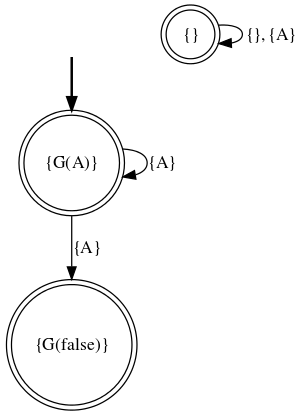
\includegraphics[width=.4\linewidth]{images/ltlf-alwaysA-nfa}
		\caption{The \NFA associated to $\Box A$.  $G(A)$ stands for $\Box A$}\label{fig:nfa-always-a}
	\end{figure}
	\begin{figure}[h!]
		\centering
		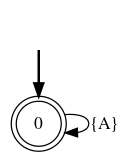
\includegraphics[width=.2\linewidth]{images/ltlf-alwaysA-dfa}
		\caption{The \DFA associated to $\Box A$}\label{fig:dfa-always-a}
	\end{figure}

	
\end{example}
\begin{example}\label{ldl2nfa-example-eventually}
	Analogously to what we did in \ref{ldl2nfa-example-always}, we see a run of the Algorithm \ref{alg:ldl2nfa}, with the \LTLf formula $\Diamond A$ ($A$ atomic).
	\begin{enumerate}
		\setcounter{enumi}{-1}
		\item Set up:
		\begin{align*}
		q_0 &= \set{\Diamond A}		\\
		Q &= \set{q_0, \emptyset}  \\
		F &= \set{\emptyset}  \ind \tm{(because $\DfunEps{\Diamond A}= \DfunEps{\true \lUntil A} = \false$)}\\
		\delta &= \set{(\emptyset, \set{}, \emptyset), (\emptyset, \set{A}, \emptyset)}
		\end{align*}
		\item \label{exa:eventually-A_it-1} Iteration: analyze $q = \set{\Diamond A}$
		\begin{itemize}
			\item \label{exa:eventually-A_it-1_prop-A} with $\PropInt = \set{A}$ we have 
			\begin{align*}
			q' &\models \bigwedge_{(\psi\in q)} \Dfun{\psi}\\
			&\models \Dfun{\Diamond A}\\
			&\models \Dfun{A} \lOR \Dfun{\Next \Diamond A}\\
			&\models \true \lOR (``\Diamond A" \lAND ``\Diamond \true")
			\end{align*}
			Since the propositional formula is trivially true, as a minimal interpretation we have $q' = \emptyset$.
			Considering that the empty conjunction is considered as $\true$ (as explained in Section \ref{sect:llf2automata}), at the end of the iteration we have:
			\begin{align*}
			q_0 &= \set{\Diamond A}		\\
			Q &= \set{q_0, \emptyset}  \\
			F &= \set{\emptyset}  \\
			\delta &= \set{(\emptyset, \set{}, \emptyset), (\emptyset, \set{A}, \emptyset), (q_0, \set{A}, \emptyset)}
			\end{align*}
			
			\item \label{exa:eventually-A_it-1_prop-empty} with $\PropInt = \set{}$ we have 
			\begin{align*}
			q' &\models \bigwedge_{(\psi\in q)} \Dfun{\psi}\\
			&\models \Dfun{\Diamond A}\\
			&\models \Dfun{A} \lOR \Dfun{\Next \Diamond A}\\
			&\models \false \lOR (``\Diamond A" \lAND ``\Diamond \true")
			\end{align*}
			As a minimal interpretation we have $q' = \set{``\Diamond A", ``\Diamond \true"}$. Since $\DfunEps{\Diamond A} \lAND \DfunEps{\Diamond \true} = \false \lAND \false \neq \true$, we do not add $q'$ to the accepting states $F$. Thus we have:
			\begin{align*}
			q_0 &= \set{\Diamond A}		\\
			Q &= \set{q_0, \emptyset, \set{\Diamond A, \Diamond \true}}  \\
			F &= \set{\emptyset}  \\
			\delta &= \set{(\emptyset, \set{}, \emptyset), (\emptyset, \set{A}, \emptyset),\\
				&\ind (q_0, \set{A}, \emptyset),\\
				&\ind (q_0, \set{}, \set{\Diamond A, \Diamond \true})}
			\end{align*}
		\end{itemize}
		
		\item \label{exa:eventually-A_it-2} Iteration: we already analyzed $q = \set{\Diamond A}$, so we analyze $q = \set{\Diamond A, \Diamond \true}$
		\begin{itemize}			
			\item with $\PropInt = \set{}$ we have that:
			\begin{align*}
			q' &\models \bigwedge_{(\psi\in q)} \Dfun{\psi}\\
			&\models \Dfun{\Diamond A} \lAND \Dfun{\Diamond \true}\\
			&\models [\Dfun{A} \lOR \Dfun{\Next \Diamond A}] \lAND [\Dfun{\true} \lOR \Dfun{\Next \Diamond true}]\\
			&\models [\Dfun{A} \lOR ( ``\Diamond A" \lAND ``\Diamond \true")] \lAND [\true \lOR ( ``\Diamond \true" \lAND ``\Diamond \true")]\\
			&\models \Dfun{A} \lOR ( ``\Diamond A" \lAND ``\Diamond \true")\\
			&\models \false \lOR ( ``\Diamond A" \lAND ``\Diamond \true")\\
			\end{align*}
			As in the previous iteration, the minimal model is $q' = \set{``\Diamond A", ``\Diamond \true"}$. Hence we add a new transition $(\set{\Diamond A, \Diamond \true}, \set{}, \set{\Diamond A,  \Diamond \true})$.

			\item with $\PropInt = \set{A}$ the delta-expansion is the same, except for the last step, where:
			\[
			q' \models \true \lOR ( ``\Diamond A" \lAND ``\Diamond \true")\
			\]
			The formula is always true, hence the minimal model is $q'=\emptyset$ and we add a new transition $(\set{\Diamond A, \Diamond \true}, \set{}. \emptyset)$. 
			
		\end{itemize}
	
	The NFA $\automaton_\varphi$ is then composed by:
	\begin{align*}
	q_0 &= \set{\Diamond A}		\\
	Q &= \set{q_0, \emptyset, \set{\Diamond A, \Diamond \true}}  \\
	F &= \set{\emptyset}  \\
	\delta &= \set{(\emptyset, \set{}, \emptyset), (\emptyset, \set{A}, \emptyset),\\
		&\ind (q_0, \set{A}, \emptyset),\\
		&\ind (q_0, \set{}, \set{\Diamond A, \Diamond \true})\\
		&\ind (\set{\Diamond A, \Diamond \true}, \set{}, \set{\Diamond A, \Diamond \true})\\
		&\ind (\set{\Diamond A, \Diamond \true}, \set{}, \emptyset)}
	\end{align*}
	\end{enumerate}
	
	The \NFA $\automaton_\varphi = \tup{2^{\set{A}}, Q, q_0, \delta, F}$ is depicted in Figure \ref{fig:nfa-eventually-a}, whereas the associated \DFA is in Figure \ref{fig:dfa-eventually-a}.
	
	\begin{figure}[h!]
		\centering
		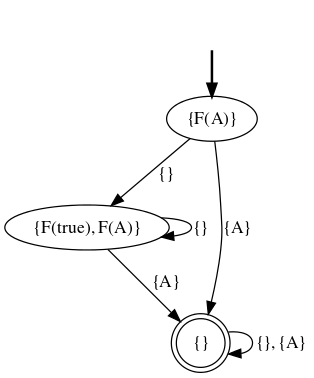
\includegraphics[width=.4\linewidth]{images/ltlf-eventuallyA-nfa}
		\caption{The \NFA associated to $\Diamond A$. $F(A)$ stands for $\Diamond A$}\label{fig:nfa-eventually-a}
	\end{figure}
	\begin{figure}[h!]
		\centering
		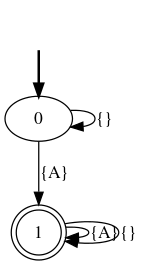
\includegraphics[width=.3\linewidth]{images/ltlf-eventuallyA-dfa}
		\caption{The \DFA associated to $\Diamond A$}\label{fig:dfa-eventually-a}
	\end{figure}
	
\end{example}

\begin{example}
	We list other examples of $\automaton_\varphi$ given a \LLf formula $\varphi$, obtained by Algorithm \ref{alg:ldl2nfa}:
	\begin{itemize}
		\item \emph{Conditional Response}: the \LTLf formula $\varphi = \Box (A \Rightarrow \Diamond B)$ or equivalently the \LDLf formula $\varphi = \BOX{\true^*}(\DIAM{A}tt \Rightarrow \DIAM{\true^*}\DIAM{B}tt)$ translates into the automaton depicted in Figure \ref{conditional-response-dfa}.
		\begin{figure}[h!]
			\centering
			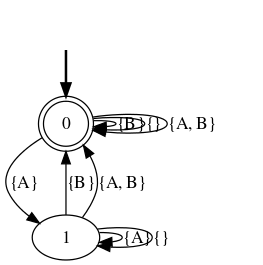
\includegraphics[width=.4\linewidth]{images/conditional-response-dfa}
			\caption{The \DFA associated to $\varphi = \Box (A \Rightarrow \Diamond B)$}\label{conditional-response-dfa}
		\end{figure}
		
		\item \emph{Alternating sequence}: the \LDLf formula $\varphi = \DIAM{(A;B)^*}\Ended$ translates into the automaton depicted in Figure \ref{alternating-sequence-dfa}.
		\begin{figure}[h!]
			\centering
			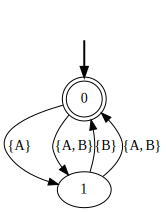
\includegraphics[width=.4\linewidth]{images/alternating-sequence-dfa}
			\caption{The \DFA associated to $\varphi = \DIAM{(A;B)^*}\Ended$}\label{alternating-sequence-dfa}
		\end{figure}
		
	\end{itemize}
\end{example}

\section{On-the-fly \DFA}
In this section, we describe a way to evaluate a \LLf formula without the need to build the entire automaton $\automaton_\varphi$. After that, we devise a new algorithm, a variant of \LDLfToNFA, that avoids the computation of the \NFA, but directly translate the formula into a \DFA. We provide some examples to clarify the presented topics.

\subsection{On-the-fly \LLf evaluation}\label{sect:on-the-fly-dfa}
In this section, we describe an alternative method to evaluate a trace on a \DFA without the need for constructing $\automaton_\varphi$, that we call \emph{on-the-fly} \citep{AAAI1817342}. The idea is, we progress all possible states that the \NFA can be in, after consuming the next trace symbol, and accept the trace iff, once it has been completely read, the set of possible states contains a final state.

More formally, call a set of possible
states for the \NFA a macrostate, let $Q = \set{q_1, \dots, q_n}$ be the current macrostate (initially $Q = Q_0 = \set{q_0} = \set{\set{\varphi}}$), and
let $\PropInt$ be the next trace symbol. Then, the successor macrostate is the set $Q'$ defined as follows: 
\begin{equation}\label{eq:on-the-fly-progression-rule}
Q' = \set{q' | \exists q \in Q\ s.t.\ q' \models \bigwedge_{(\psi \in q)} \DfunSym(\psi, \PropInt)}
\end{equation} Notice that the condition $q' \models \bigwedge_{(\psi \in q)} \DfunSym(\psi, \PropInt)$ is the same of the one in line \ref{ldlf2nfa:delta-for-loop} of Algorithm \ref{alg:ldl2nfa}.
Given an input trace $\trace$, we decide whether $\trace \models \varphi$ by iterating
the above procedure, starting from the initial state $Q = Q_0$,
and accepting $\trace$ iff the last state obtained includes $\set{\true}$, considering their evaluation in the empty trace (i.e. with $\DfunEps{\psi}$). We denote the evaluation over the empty trace of a macrostate $Q = \set{q_1, \dots, q_n}$ as $Q^\epsilon$. Formally:
\begin{equation}\label{eq:macro-state-epsilon}
Q^\epsilon = \set{\varphi | \varphi = \bigwedge_{\psi\in q_i} \DfunEps{\psi}}
\end{equation}

\begin{example}\label{exa:on-the-fly-always-A}
	Consider Example \ref{ldl2nfa-example-always} with $\varphi = \Box A$, we show how the on-the-fly evaluation of traces works.
	At the beginning, we have that $$Q = Q_0 = \set{\set{\Box A}}$$

	In this example, we ask the following questions:
	\begin{enumerate}
		\item $\tup{} \models \varphi$? Does the empty trace $\trace = \tup{}$ satisfy the formula $\varphi$? We expect that the answer is yes, due to the semantics of $\Box A$. With the on-the-fly approach, we need to compute for each \NFA state $q \in Q$ the conjunction between every $\DfunEps{\psi}$, where $\psi \in q$. As said before, we consider the empty conjunction as $\set{\true}$.
		
		In our example, the computation gives us:
		$$Q_0^\epsilon = \set{\set{\true}}$$
		because $\DfunEps{\Box A} = \true$.
		Since $Q_0^\epsilon$ contains $\set{\true}$, $Q_0^\epsilon$ is an accepting state, hence $\trace \models \Box A$, as expected.
		
		\item $\tup{\set{}} \models \varphi$? This time consider the trace $\trace = \tup{\set{}}$ or, equivalently, $\trace = \tup{\lnot A}$. We expect that the on-the-fly evaluation returns $\false$, hence $\trace \not \models \varphi$. In order to answer, we need to progress the automaton on-the-fly for each element of the trace (in this case only one) and check if the last macrostate is an accepting state by using the procedure explained in the previous case.
		The next macrostate $Q_1$ by applying Equation \ref{eq:on-the-fly-progression-rule}. Actually, it is computed as we did in Iteration \ref{exa:always-A_it-1_prop-empty} of Example \ref{ldl2nfa-example-always} with $\PropInt = \set{}$. 
		
		Since no $q'$ can be found, $Q_1 = \set{}$, which is not an accepting state since $\set{\true} \notin Q_1^\epsilon$. Hence, $\trace \not \models \varphi$.\label{exa:on-the-fly-always-A-trace-false}
		
		\item \label{exa:on-the-fly-always-A-trace-A} $\tup{\set{A}} \models \varphi$? Consider the trace $\trace = \tup{\set{}}$. We expect that the on-the-fly evaluation returns $\true$, hence $\trace \models \varphi$. We proceed, as in the previous case, to compute the next macrostate $Q_1$ by applying Equation \ref{eq:on-the-fly-progression-rule}. Actually, it is computed as we did in Iteration \ref{exa:always-A_it-1_prop-A} with $\PropInt = \set{A}$. As a minimal interpretation we have both $q' = \set{\Box A}$ and $q' = \set{\Box \false}$. Hence, the new macrostate is $Q_1 = \set{\set{\Box A}, \set{\Box \false}}$.
		
		Since there are no other symbols in the trace $\trace$ to be processed, we compute $Q_1^\epsilon = \set{\set{true}, \set{true}} = \set{\set{true}}$. Since $\set{true} \in Q_1^\epsilon$, we can say that $\trace \models \varphi$.
		
		\item $\tup{\set{A}, \set{}} \models \varphi$? Consider the trace $\trace = \tup{\set{A}, \set{}}$. We expect that the on-the-fly evaluation returns $\false$, hence $\trace \not\models \varphi$. We proceed, as in the previous case, to compute the next macrostates by applying Equation \ref{eq:on-the-fly-progression-rule}. Macrostate $Q_1$ is the same as we have seen in Case \ref{exa:on-the-fly-always-A-trace-A}. 
		We apply again the progression rule of Equation \ref{eq:on-the-fly-progression-rule} with $\PropInt = \trace(2) = \set{}$. 
		As a minimal interpretation we have both $q' = \set{\Box A}$ and $q' = \set{\Box \false}$. Hence, the new macrostate is $Q_2 = \set{}$. as we've seen in Iteration \ref{exa:always-A_it-2} of Example \ref{ldl2nfa-example-always}.
		
		Since there are no other symbols in the trace $\trace$ to be processed, we compute $Q_2^\epsilon = \set{}$. Since $\set{true} \not\in Q_2^\epsilon$, we can say that $\trace \not\models \varphi$.
		
		\item $\tup{\set{}, \set{A}} \models \varphi$? Consider the trace $\trace = \tup{\set{}, \set{A}}$. We expect that the on-the-fly evaluation returns $\false$, hence $\trace \not\models \varphi$. The macrostate $Q_1$ is the same as we have seen in Case \ref{exa:on-the-fly-always-A-trace-false}, i.e. $Q_1 = \set{}$. 
		We apply again the progression rule of Equation \ref{eq:on-the-fly-progression-rule} with $\PropInt = \trace(2) = \set{A}$. But this is trivially $Q_2 = \set{}$, by definition of the progression rule.
		
		Since there are no other symbols in the trace $\trace$ to be processed, we compute $Q_2^\epsilon = \set{}$. Since $\set{true} \not\in Q_2^\epsilon$, we can say that $\trace \not\models \varphi$.
		
	\end{enumerate}	
	Notice how we use the same progression of Algorithm \ref{alg:ldl2nfa}, but instead of aiming to build the entire automaton, we focus only on the states that are relevant for the satisfaction of the formula, given a trace.
	
\end{example}

\begin{example}\label{exa:on-the-fly-eventually-A}
	Analogously as we did in Example \ref{exa:on-the-fly-always-A} for Example \ref{ldl2nfa-example-always}, we consider Example \ref{ldl2nfa-example-eventually} with $\varphi = \Diamond A$, and we show how the on-the-fly evaluation of traces works also in this case.
	At the beginning, we have that $$Q = Q_0 = \set{\set{\Diamond A}}$$
	
	In this example, we ask the following questions:
	\begin{enumerate}
		\item $\tup{} \models \varphi$? Does the empty trace $\trace = \tup{}$ satisfy the formula $\varphi$? We expect that the answer is no, due to the semantics of $\Diamond A$. 
		
		We observe that $Q_0^\epsilon = \set{}$,
		because $\DfunEps{\Diamond A} = \false$.
		
		Since $Q_0^\epsilon$ does not contain $\set{\true}$, $Q_0^\epsilon$ is not an accepting state, hence $\trace \not\models \Diamond A$, as expected.
		
		\item $\tup{\set{}} \models \varphi$? This time consider the trace $\trace = \tup{\set{}}$ or, equivalently, $\trace = \tup{\lnot A}$. We expect that the on-the-fly evaluation returns $\false$, hence $\trace \not \models \varphi$. In order to answer, we need to progress the automaton on-the-fly for each element of the trace (in this case only one) and check if the last macrostate is an accepting state by using the procedure explained in the previous case.
		The next macrostate $Q_1$ by applying Equation \ref{eq:on-the-fly-progression-rule}. Actually, it is computed as we did in Iteration \ref{exa:eventually-A_it-1_prop-empty} of Example \ref{ldl2nfa-example-eventually} with $\PropInt = \set{}$. 
		 As a minimal interpretation we have $q' = \set{\Diamond A, \Diamond \true}$. Hence, the new macrostate is $Q_1 = \set{\set{\Diamond A, \Diamond \true}}$.
		 
		Now, $Q_1^\epsilon = \set{\set{\false}}$, which is not an accepting state since $\set{\true} \notin Q_1^\epsilon$. Hence, $\trace \not \models \varphi$.\label{exa:on-the-fly-eventually-A-trace-false}
		
		\item $\tup{\set{A}} \models \varphi$? Consider the trace $\trace = \tup{\set{}}$. We expect that the on-the-fly evaluation returns $\true$, hence $\trace \models \varphi$. We proceed, as in the previous case, to compute the next macrostate $Q_1$ by applying Equation \ref{eq:on-the-fly-progression-rule}. Actually, it is computed as we did in Iteration \ref{exa:eventually-A_it-1_prop-A} with $\PropInt = \set{A}$. As a minimal interpretation we have $q' = \empty$. Hence, the new macrostate is $Q_1 = \set{\emptyset}$.
		
		Since there are no other symbols in the trace $\trace$ to be processed, we compute $Q_1^\epsilon = \set{\set{true}}$. Since $\set{true} \in Q_1^\epsilon$, we can say that $\trace \models \varphi$.\label{exa:on-the-fly-eventually-A-trace-A}
		
		\item $\tup{\set{A}, \set{}} \models \varphi$? Consider the trace $\trace = \tup{\set{A}, \set{}}$. We expect that the on-the-fly evaluation returns $\true$, and so $\trace \models \varphi$. We proceed, as in the previous case, to compute the next macrostates by applying Equation \ref{eq:on-the-fly-progression-rule}. Macrostate $Q_1$ is the same as we have seen in Case \ref{exa:on-the-fly-eventually-A-trace-A}. 
		We apply again the progression rule of Equation \ref{eq:on-the-fly-progression-rule} with $\PropInt = \trace(2) = \set{}$, that leads to the new macrostate is $Q_2 = \set{\emptyset}$. Notice that $Q_1 = Q_2$.
		
		Since there are no other symbols in the trace $\trace$ to be processed, we compute $Q_2^\epsilon = \set{\set{\true}}$. Since $\set{true} \in Q_2^\epsilon$, we can say that $\trace \models \varphi$.
		
		\item \label{exa:on-the-fly-eventually-A-trace-false-A}$\tup{\set{}, \set{A}} \models \varphi$? Consider the trace $\trace = \tup{\set{}, \set{A}}$. We expect that the on-the-fly evaluation returns $\true$, hence $\trace \models \varphi$. The macrostate $Q_1$ is the same as we have seen in Case \ref{exa:on-the-fly-eventually-A-trace-false}, i.e. $Q_1 = \set{\set{\Diamond A, \Diamond \true}}$. 
		We apply again the progression rule of Equation \ref{eq:on-the-fly-progression-rule} with $\PropInt = \trace(2) = \set{A}$. But this is trivially $Q_2 = \set{\emptyset}$ (as we've seen in Iteration \ref{exa:eventually-A_it-2} of Example \ref{ldl2nfa-example-eventually}), by definition of the progression rule.
		
		Since there are no other symbols in the trace $\trace$ to be processed, we compute $Q_2^\epsilon = \set{\set{\true}}$. Since $\set{\true} \in Q_2^\epsilon$, we can say that $\trace \models \varphi$.
		
	\end{enumerate}	
	Notice how we use the same progression  of Algorithm \ref{alg:ldl2nfa}, but instead of aiming to build the entire automaton, we focus only on the states that are relevant for the satisfaction of the formula, given a trace.
	
\end{example}

\subsection{\LDLfToDFA: a variant of \LDLfToNFA}\label{sect:llf2dfa}

Example \ref{exa:on-the-fly-always-A} and \ref{exa:on-the-fly-eventually-A} suggest a new way to translate \LLf formulas to automata, that is a variant of \LDLfToNFA (Algorithm \ref{alg:ldl2nfa}). We call it \LDLfToDFA, and directly translates a \LLf formula to a \DFA, instead of first translation into a \NFA and then compute the \DFA by determinization.

\begin{algorithm}
	\caption{\LDLfToDFA: from \LTLf/\LDLf formula $\varphi$ to \DFA $\automaton_\varphi$}
	\label{alg:ldlf2dfa}
	\begin{algorithmic}[1]
		\State \algInput\ \LDLf/\LTLf formula $\varphi$
		\State \algOutput\ \DFA $\automaton_\varphi = \tup{2^\Prop, \Q, Q_0, \delta, F}$ \Comment Notice: $\Q$ is a set of macrostates.
		
		\State $Q_0 \gets \set{\set{\varphi}}$ \Comment the initial state of $\automaton_\varphi$ is the initial macrostate
		\State $F \gets \emptyset$
		\State $\Q \gets \set{Q_0}$
		\State $\delta \gets \emptyset$
		\If{$(\set{\true}\in Q_0^\epsilon)$} \label{ldlf2dfa:delta-eps-init}
			\State $F \gets F \cup \set{Q_0}$
		\EndIf
		
		\While{$(\Q \tm{or} \delta\ \text{change})$}
			\For{$(Q\in \Q, \PropInt\in2^\Prop)$}
				\State $Q' \gets \set{}$
				\For{$(q \in Q)$} \label{ldlf2dfa:main-for-loop}\Comment Conceptually, the same loop of Algorithm \ref{alg:ldl2nfa}, line \ref{ldlf2nfa:main-for-loop}
					\If{$(q'\models \bigwedge_{(\psi\in q)} \Dfun{\psi})$} \label{ldlf2dfa:delta-for-loop}
						\State $Q' \gets Q' \cup \set{q'}$
					\EndIf
				\EndFor
				\State $\Q \gets \Q \cup \set{Q'}$ \Comment Add new macrostate  $Q$ to the set of macrostates $\Q$
				\State $\delta \gets \delta \cup \set{(Q, \PropInt, Q')}$
				\If{$(\set{\true}\in Q'^\epsilon)$} \label{ldlf2dfa:delta-eps-end}
					\State $F \gets F \cup \set{Q'}$
				\EndIf
			\EndFor
		
		\EndWhile
%		\State Minimize $\automaton_\varphi$
		
	\end{algorithmic}
	
\end{algorithm}
The idea behind Algorithm \ref{alg:ldlf2dfa} is the following: build the \DFA by doing the exploration of automaton states and determinization \emph{at the same time}. Indeed, each macrostate tracks all the possible paths (according to the trace symbols processed) of the "implicit" \NFA. The computation of the next \NFA state, i.e. the for-loop at line \ref{ldlf2dfa:main-for-loop}, works in the same way of the for-loop in line \ref{ldlf2nfa:main-for-loop} of Algorithm \ref{alg:ldl2nfa}. For a single macrostate $Q$, given a propositional interpretation $\PropInt$, the operation is made for every \NFA state $q\in Q$. The next macrostate $Q'$ is then composed by all the next \NFA states $q'$. Given the triple $Q, \PropInt, Q'$, we actually have a transition of the \DFA $\automaton_\varphi$. Doing this operation for every macrostate and for every interpretation, until convergence, will eventually lead to the exploration of every macrostate and transitions among them. 

The main advantage over Algorithm \ref{alg:ldl2nfa} is that we avoid the state explosion due to the determinization procedure since we only process reachable states of the final \DFA. We use this algorithm in the implementations of Chapter \ref{ch:flloat}.

\begin{example}
	We consider Example \ref{ldl2nfa-example-always} but using Algorithm \ref{alg:ldlf2dfa} for translation of $\varphi = \Box A$ into a \DFA.
	
	\begin{enumerate}
		\setcounter{enumi}{-1}
		\item Before the main loop, we have:
			\begin{align*}
			Q_0 &= \set{\set{\Box A}}\\
			\Q  &= \set{Q_0}\\
			\delta &= \emptyset\\
			F &= \set{Q_0} \ind (\text{because } \set{true}\in Q_0^\epsilon)
			\end{align*}
		The \DFA at this stage is depicted in Figure \ref{fig:exa-on-the-fly-always-A-it-0}.
		
		\item Iteration: Consider the macrostate $Q_0$. Consider the (unique) \NFA state $\set{\Box A}$. 
		
		With $\PropInt = \set{A}$ we generate the new macrostate $Q' = \set{\set{\Box A}, \set{\Box \false}}$. We add $Q'$ to $\Q$ and $(Q_0, \PropInt, Q')$ to $\delta$. We followed the same steps as we did in Example \ref{exa:on-the-fly-always-A}, Case \ref{exa:on-the-fly-always-A-trace-A}.
		
		With $\PropInt = \set{}$ we generate the new macrostate $Q' =\emptyset$.  We add $Q'$ to $\Q$ and $(Q_0, \PropInt, Q')$ to $\delta$. Since $\set{\true}\not\in\Q'^\epsilon$, we do not add $Q'$ to $F$. We followed the same steps as we did in Example \ref{exa:on-the-fly-always-A}, Case \ref{exa:on-the-fly-always-A-trace-false}.
		
		\medskip
		
		The \DFA at this stage is depicted in Figure \ref{fig:exa-on-the-fly-always-A-it-1}.
		
		\item Iteration: We already processed $Q=\set{\set{\Box A}}$.
		
		Consider the macrostate $Q = \emptyset$. Since there exists no $q\in Q$, the for-loop at line \ref{ldlf2dfa:main-for-loop}, we add to $\delta$ all the transitions of the form $(\emptyset, \PropInt, \emptyset)$, for all $\PropInt \in 2^\Prop$.
 
		 Now consider the macrostate $Q = \set{\set{\Box A}, \set{\Box \false}}$. 
		
		Consider $\PropInt = \set{A}$. For $q = \set{\Box A}$ we generate the sub-macrostate $q' = \set{\Box A}$ and $q' = \set{\Box \false}$. For $q = \set{\Box \false}$ we do not generate any sub-macrostate.
		Hence, the resulting macrostate is $Q' = \set{\set{\Box A}, \set{\Box \false}}$. Since $Q'\in \Q$, we only add $(Q, \PropInt, Q')$ to $\delta$.
		
		Consider $\PropInt = \set{}$. For $q = \set{\Box A}$ we do not generate any sub-macrostate. For $q = \set{\Box \false}$ we do not generate any sub-macrostate.
		Hence, the resulting macrostate is $Q' = \set{}$. Since $Q'\in \Q$, we only add $(Q, \PropInt, Q')$ to $\delta$.
		 
		Since there are no other macrostates nor propositional interpretation to process, the algorithm terminates. The final \DFA is depicted in Figure \ref{fig:exa-on-the-fly-always-A-it-complete}.
		
	\end{enumerate}

\begin{figure}[h]
	\centering
	\begin{subfigure}[b]{0.20\textwidth}
		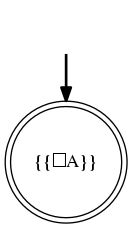
\includegraphics[width=\textwidth]{images/on-the-fly-always-A-it-0}
			 	\caption{Iteration 0}
			 	\label{fig:exa-on-the-fly-always-A-it-0}
	\end{subfigure}
	~ %add desired spacing between images, e. g. ~, \quad, \qquad, \hfill etc. 
	%(or a blank line to force the subfigure onto a new line)
	\begin{subfigure}[b]{0.35\textwidth}
		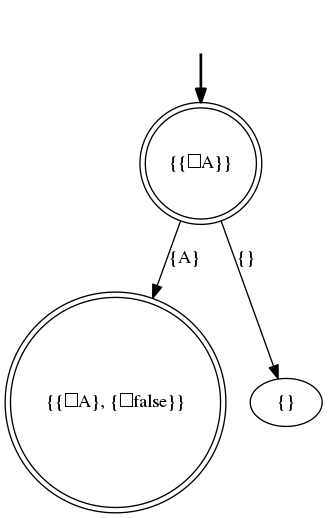
\includegraphics[width=\textwidth]{images/on-the-fly-always-A-it-1}
		\caption{Iteration 1}
		\label{fig:exa-on-the-fly-always-A-it-1}
	\end{subfigure}
	
	\begin{subfigure}[b]{0.35\textwidth}
		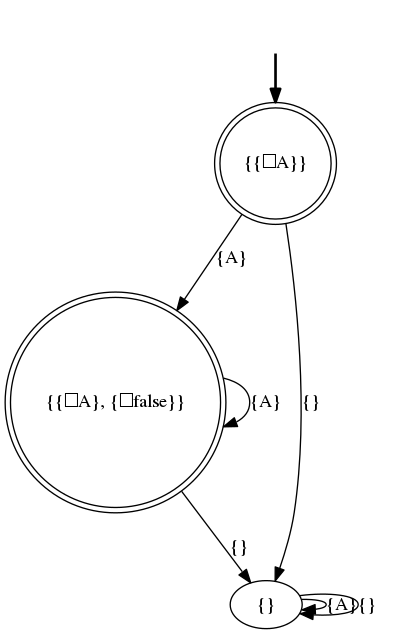
\includegraphics[width=\textwidth]{images/on-the-fly-always-A-it-complete}
		\caption{Iteration 2}
		\label{fig:exa-on-the-fly-always-A-it-complete}
	\end{subfigure}
	\caption{The automaton of Example \ref{exa:on-the-fly-always-A}, step by step.}\label{fig:exa-on-the-fly-always-A}
\end{figure}

It is interesting to observe that the macrostate $Q = \set{\set{\Box A}, \set{\Box \false}}$, where we end after reading the symbol $\set{A}$ from the initial state, is the set of \NFA states (Figure \ref{fig:nfa-always-a}) where we could ends after reading the same symbol from the initial state, namely $\set{\Box A}$ and $\set{\Box \false}$. Analogous considerations can be made for other symbols and other macrostates.

This observation makes clearer the true meaning of Algorithm \ref{alg:ldlf2dfa} with respect to Algorithm \ref{alg:ldl2nfa}: that is, the macrostates keep track of all the possible evolutions of the \NFA with respect to a trace $\trace$. By reading all the possible symbols from every macrostate, we will eventually discover all the relevant states of the \DFA.

Furthermore, the minimization and trimming of the resulting automaton (shown in Figure \ref{fig:exa-on-the-fly-always-A-it-complete}) yield the one shown in Figure \ref{fig:dfa-always-a}, as an evidence of the equivalence between the two algorithms.
\end{example}

\clearpage
\begin{example}
	We consider Example \ref{ldl2nfa-example-eventually} but using Algorithm \ref{alg:ldlf2dfa} for translation of $\varphi = \Diamond A$ into a \DFA.
	
	\begin{enumerate}
		\setcounter{enumi}{-1}
		\item Before the main loop, we have:
		\begin{align*}
		Q_0 &= \set{\set{\Diamond A}}\\
		\Q  &= \set{Q_0, \emptyset}\\
		\delta &= \emptyset\\
		F &= \emptyset \ind (\text{because } \set{true}\not\in Q_0^\epsilon)
		\end{align*}
		The \DFA at this stage is depicted in Figure \ref{fig:exa-on-the-fly-eventually-A-it-0}.
		
		\item Iteration: Consider the macrostate $Q_0$. Consider the (unique) \NFA state $\set{\Diamond A}$. 
		
		With $\PropInt = \set{A}$ we generate the new macrostate $Q' = \set{\emptyset}$. We add $Q'$ to $\Q$ and $(Q_0, \PropInt, Q')$ to $\delta$. Since $\set{\true}\in\Q'^\epsilon$, we add $Q'$ to $F$. We followed the same steps as we did in Example \ref{exa:on-the-fly-eventually-A}, Case \ref{exa:on-the-fly-eventually-A-trace-A}.
		
		With $\PropInt = \set{}$ we generate the new macrostate $Q' =\set{\set{\Diamond A, \Diamond \true}}$. We add $Q'$ to $\Q$ and $(Q_0, \PropInt, Q')$ to $\delta$. Since $\set{\true}\not\in\Q'^\epsilon$, we do not add $Q'$ to $F$. We followed the same steps as we did in Example \ref{exa:on-the-fly-eventually-A}, Case \ref{exa:on-the-fly-eventually-A-trace-false}.
		
		The \DFA at this stage is depicted in Figure \ref{fig:exa-on-the-fly-eventually-A-it-1}.
		
		\item Iteration: We already processed $Q=\set{\set{\Box A}}$.
		
		Consider the macrostate $Q = \set{\emptyset}$. Since 
		the unique successor state of $q=\emptyset$ is $q'=\emptyset$, the next macrostate, for every symbol, is the same. Hence, we add to $\delta$ all the transitions of the form $(\set{\emptyset}, \PropInt, \set{\emptyset})$, for all $\PropInt \in 2^\Prop$.
		
		Now consider the macrostate $Q = \set{\set{\Diamond A, \Diamond \true}}$. 
		
		Consider $\PropInt = \set{A}$. As we've seen in Case \ref{exa:on-the-fly-eventually-A-trace-false-A} of Example \ref{exa:on-the-fly-eventually-A}, the next macrostate is $Q'=\set{\emptyset}$, since that for $q = \set{\Diamond A, \Diamond \true}$ the successor state is $q'=\emptyset$. Since $Q'\in \Q$, we only add $(Q, \PropInt, Q')$ to $\delta$.
		
		Consider $\PropInt = \set{}$. The successor state of $q = \set{\Diamond A, \Diamond \true}$ is $q' = q$.
		Hence, the resulting macrostate is $Q' = \set{\set{\Diamond A, \Diamond \true}}$. Since $Q'\in \Q$, we only add $(Q, \PropInt, Q')$ to $\delta$. We followed the same steps as we did in Example \ref{ldl2nfa-example-eventually}, Iteration  \ref{exa:eventually-A_it-2}.
		
		Since there are no other macrostates nor propositional interpretation to process, the algorithm terminates. The final \DFA is depicted in Figure \ref{fig:exa-on-the-fly-eventually-A-it-complete}.
		
	\end{enumerate}
	
	\begin{figure}[h]
		\centering
		\begin{subfigure}[b]{0.17\textwidth}
			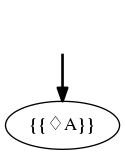
\includegraphics[width=\textwidth]{images/on-the-fly-eventually-A-it-0}
			\caption{Iteration 0}
			\label{fig:exa-on-the-fly-eventually-A-it-0}
		\end{subfigure}
		~ %add desired spacing between images, e. g. ~, \quad, \qquad, \hfill etc. 
		%(or a blank line to force the subfigure onto a new line)
		\begin{subfigure}[b]{0.50\textwidth}
			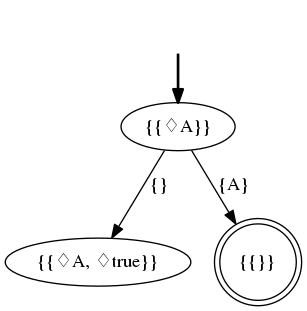
\includegraphics[width=\textwidth]{images/on-the-fly-eventually-A-it-1}
			\caption{Iteration 1}
			\label{fig:exa-on-the-fly-eventually-A-it-1}
		\end{subfigure}
		
		\begin{subfigure}[b]{0.5\textwidth}
			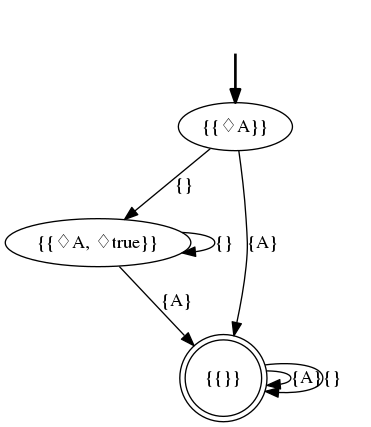
\includegraphics[width=\textwidth]{images/on-the-fly-eventually-A-it-complete}
			\caption{Iteration 2}
			\label{fig:exa-on-the-fly-eventually-A-it-complete}
		\end{subfigure}
		\caption{The automaton of Example \ref{exa:on-the-fly-eventually-A}, step by step.}\label{fig:exa-on-the-fly-eventually-A}
	\end{figure}
	
	
\end{example}


\section{Reasoning in \LLf}
In this section, we study the complexity of \LLf reasoning (i.e. complexity of problems as defined in Definition \ref{ltlf-sat-val-ent}, by leveraging the automata construction described in previous sections.

\begin{theorem}[\cite{de2013linear}] Satisfiability, validity, and logical implication for \LDLf formulas are \PSPACE-complete
\end{theorem}
\begin{proof}
	Given a \LLf $\varphi$, we can leverage Theorem \ref{ldlf2nfa-correctness} to solve these problems, namely:
	\begin{itemize}
		\item For \LLf satisfiability we compute the associated \NFA (as explained in Section \ref{sect:llf2automata} (which is an exponential step) and then check \NFA for nonemptiness (\NLOGSPACE).
		\item For \LLf validity we compute the \NFA associated to $\lnot \varphi$ (which is an exponential step) and then check \NFA for nonemptiness (\NLOGSPACE).
		\item For \LLf logical implication $\psi \models \varphi$ we compute the \NFA associated to $\psi \wedge \lnot \varphi$ (which is an exponential step) and then check \NFA for nonemptiness (\NLOGSPACE).
	\end{itemize}
\end{proof}

%TODO ON-THE-FLY

\section{Conclusions}
In this chapter, we provided the logical tools to face other topics in later chapters. We introduced several formal languages that allowed us to introduce \LTLf and \LDLf, focusing on their interesting properties. Moreover, we described in detail the procedure for translation from \LLf formulas to \DFAs, which yields an effective way of reasoning about \LLf formulas.
